\documentclass[11pt]{article}

\usepackage{amsmath}
\usepackage{amssymb}
\usepackage{geometry}
\usepackage{tikz}
\usetikzlibrary{shapes,arrows,positioning}
\usepackage{booktabs}
\usepackage{graphicx}
\usepackage{subcaption}
\usepackage{multirow}
\usepackage{lineno}

\begin{document}

\linenumbers

\title{An Interpretable Statistical Surrogate of Activated Sludge Systems that Preserves Mass Conservation and Component Non-Negativity}
\author{}

\maketitle

\section*{Nomenclature}
\begin{tabbing}
\hspace{2.5cm} \= \kill
$A$ \> Full-row-rank invariant matrix defining the null space of the stoichiometric matrix \\
$B$ \> Second-order driver coefficient matrix \\
$c_{aff}$ \> Invariant-consistent affine correction used before constrained deployment \\
$c_{in}$ \> Influent ASM component concentration vector ($c_{in} \in \mathbb{R}^{F}$) \\
$c_{out}$ \> True steady-state effluent ASM component concentration vector ($c_{out} \in \mathbb{R}^{F}$) \\
$c_{raw}$ \> Unconstrained coupled component prediction before affine presolve \\
$\hat{c}$ \> Final deployed ICSOR ASM component prediction \\
$\widehat{C}$ \> Fitted non-negative component prediction matrix used in training \\
$D$ \> Total dimension of the second-order feature map \\
$F$ \> Number of mechanistic ASM components \\
$\Gamma$ \> Learned ASM component coupling matrix \\
$I_{comp}$ \> Composition matrix mapping ASM components to measured composites ($I_{comp} \in \mathbb{R}^{K \times F}$) \\
$K$ \> Number of measured composite variables \\
$\lambda_B$ \> Ridge regularization weight on $B$ \\
$\lambda_\Gamma$ \> Ridge regularization weight on $\Gamma$ \\
$\lambda_{inv}$ \> Invariant-residual penalty weight in the training objective \\
$\lambda_{sys}$ \> Coupled-system consistency penalty weight in the training objective \\
$M_{op}$ \> Number of operational variables \\
$N_{rxn}$ \> Number of reactions in the mechanistic model \\
$R$ \> Coupled-system matrix, $R = I_F - \Gamma$ \\
$u$ \> Operational input vector ($u \in \mathbb{R}^{M_{op}}$) \\
$w_c$ \> Componentwise weight vector used in deployed correction \\
$y_{ext}$ \> Reported measured effluent composite vector ($y_{ext} \in \mathbb{R}^{K}$) \\
$\hat{y}_{ext}$ \> Reported composite prediction, $\hat{y}_{ext} = I_{comp}\hat{c}$ \\
$\nu$ \> Stoichiometric matrix ($\nu \in \mathbb{R}^{N_{rxn} \times F}$) \\
$\xi$ \> Net reaction progress vector \\
$\phi$ \> Partitioned second-order feature map \\
$\otimes$ \> Kronecker product \\
\end{tabbing}

\section{Introduction}

Water pollution presents a critical environmental and public health challenge worldwide, with particularly severe repercussions in developing nations (Lin et al., 2022; Madhav et al., 2020). Biological wastewater treatment systems, particularly those based on the activated sludge process, are the dominant approach applied to combat this issue (Duan et al., 2022). However, their modeling and analysis present formidable engineering and computational challenges (Xiao et al., 2025). The underlying biophysical mechanisms are governed by the Activated Sludge Models (ASM) (Henze et al., 2006), which rely on coupled, multiplicative non-linear kinetic expressions to describe microbial growth and substrate consumption. This inherent non-linearity limits the practical application of transparent analytical methods for process design, frequently forcing engineers to rely on iterative trial-and-error approaches or computationally expensive heuristic algorithms (Aboagye et al., 2021; Padron-Paez et al., 2020).

In response to the computational and mathematical complexity inherent in non-linear Activated Sludge Models, research has increasingly focused on developing surrogate models to approximate the behavior of biological wastewater treatment systems (Bhosekar \& Ierapetritou, 2018; Durkin et al., 2024; Tsochatzidi et al., 2025). Traditional approaches have explored linearization techniques (Li et al., 2020; Yang et al., 2014) and multivariable polynomial fitting (Ahn et al., 2014; Kim et al., 2009; Lim et al., 2011). While linear methods like Partial Least Squares (PLS) offer interpretable mappings, they inherently struggle to capture the severe non-linearities of microbial kinetics without extensive feature engineering. To overcome these limitations, the machine learning (ML) paradigm has emerged as a powerful route for approximating highly non-linear wastewater-treatment behavior (Croll et al., 2023; Nazlabadi et al., 2021). A wide array of data-driven algorithms—ranging from distance-based methods like k-Nearest Neighbors (k-NN) and PLS (Khatri et al., 2020; Wold et al., 2001), to kernel methods like Support Vector Regression (SVR) (Fang et al., 2011), tree-based ensembles such as Random Forest (RF), AdaBoost, XGBoost, LightGBM, and CatBoost (Sadri Moghaddam \& Mesghali, 2023; Wang et al., 2025; Yang et al., 2025), and Artificial Neural Networks (ANN) (Asadi et al., 2017; Bagherzadeh et al., 2021; Mao et al., 2024)—have demonstrated strong predictive capabilities for effluent quality. 

Despite their predictive accuracy, these standard ML algorithms remain structurally blind to a central physical requirement of activated sludge systems: material cannot be created or destroyed arbitrarily across the modeled control volume. A surrogate may fit observed effluent behavior well while still implying an impossible redistribution of the underlying ASM components, thereby violating the mass balances that govern COD, nitrogen, or phosphorus transfer. At the same time, physically admissible concentration states must remain componentwise non-negative. These two requirements are inseparable in practice. A surrogate that conserves mass but predicts negative concentrations is still unusable, and a surrogate that preserves non-negativity while violating mass conservation remains physically misleading.

Recent scientific-ML literature shows that satisfying both requirements simultaneously is nontrivial. A substantial class of methods enforces conservation alone through conservative flux formulations, stoichiometric architectures, projection operators, Bayesian reconciliation, or completion strategies, but does not guarantee non-negativity of the corrected state (Beucler et al., 2021; Geiss et al., 2022; Hansen et al., 2023; Harder et al., 2022; Sturm \& Silva, 2025; Sturm \& Wexler, 2020, 2022). Closely related soft-constraint approaches, such as physics-informed neural networks, can encourage physically plausible behavior but generally provide neither exact conservation nor strict positivity guarantees (Raissi et al., 2019). Conversely, positivity-only constructions such as output transformations ensure non-negative states yet do not enforce global material balance (Kircher \& Votsmeier, 2025).

A smaller body of work has reported simultaneous enforcement of conservation and non-negativity. Kircher and Votsmeier (2025) develop positivity-preserving conservative corrections for mechanistic kinetics surrogates in atmospheric chemistry and heterogeneous catalysis. Min et al. (2024) and Utkarsh et al. (2025) propose hard-constrained learning frameworks that can impose equality and inequality constraints together in more general machine-learning settings. In atmospheric transport, Sturm et al. (2023) show that mass-preserving scaling can maintain both total conservation and non-negativity for advected aerosol superspecies. These results demonstrate that dual physical guarantees are achievable, but they arise in application settings whose state definitions, constraints, and deployment objectives differ substantially from those of activated sludge process surrogates.

This gap is consequential for wastewater engineering. Activated sludge models couple multiple conserved material inventories with biologically and chemically constrained component states, so violations of either mass conservation or non-negativity can distort interpretation, confound process optimization, and undermine confidence in surrogate-assisted design. A physically constrained data-driven model would therefore offer several practical benefits: it would preserve the bookkeeping needed for COD, nitrogen, and phosphorus analysis, prevent impossible negative component concentrations, reduce reliance on ad hoc clipping or reconciliation, and yield predictions that remain more defensible as operating conditions and influent loads vary. Yet, to our knowledge, no prior activated sludge surrogate has provided hard guarantees of both stoichiometric mass conservation and componentwise non-negativity within a single interpretable steady-state framework.

This study addresses that need through the development of Invariant-Constrained Second-Order Regression (ICSOR), a physics-informed surrogate framework for steady-state activated sludge systems. ICSOR is designed to answer a practical question: given a steady-state influent condition and operating point, what effluent state should be predicted if the surrogate is required to remain physically admissible by construction? Rather than treating physical consistency as a soft regularizer or a purely diagnostic afterthought, the framework is built so that deployed predictions satisfy both mass-conservation requirements and non-negativity requirements simultaneously.

To do so, ICSOR couples an interpretable second-order surrogate with a hard physical correction performed in ASM component space. The regression structure retains transparent operating-condition, influent, and interaction effects, while the deployment step removes states that would violate the admissible physical region. The result is a surrogate that remains analytically structured and data-driven, yet is constrained to return only physically meaningful steady-state predictions.

The objective of this article is to formulate the ICSOR framework as an analytically structured surrogate and to evaluate its efficacy on a standalone Continuous Stirred Tank Reactor (CSTR). By comparing ICSOR against established unconstrained baselines, this study assesses whether the proposed model can achieve competitive predictive accuracy while explicitly guaranteeing the parsimony, interpretability, and rigorous physical consistency required for reliable process analysis. The framework presented herein is strictly bounded to steady-state predictions; while it guarantees mass conservation and non-negativity, it does not claim to enforce full kinetic or thermodynamic feasibility, nor does it replace dynamic trajectory simulators. Instead, it occupies a necessary middle ground: a surrogate simple enough to be estimated transparently from data, yet mathematically constrained to respect the fundamental physical constraints of wastewater engineering.

\section{Theory and Calculation}

\subsection{Physical Scope, State Spaces, and Notation}

A fixed reactor block or process unit represented by steady-state samples is considered. The system boundary used to define influent and effluent states is identical to the boundary used to define stoichiometric conservation. Any external source or sink that crosses that boundary must therefore be represented in the adopted stoichiometric model; otherwise, it lies outside the present conservation claim.

ICSOR is formulated natively in ASM component space. Its scientific output is the effluent component vector itself, not a measured aggregate. Measured composites are obtained only afterward through an external composition matrix. This choice is deliberate because mass conservation and componentwise non-negativity are both defined in ASM component coordinates.

Let $M_{op}$ be the number of operational variables, $F$ the number of ASM components, $K$ the number of reported composite variables, and $N_{rxn}$ the number of reactions. Single-sample vectors are written as column vectors. The following state spaces and operators are defined:
\begin{itemize}
    \item $u \in \mathbb{R}^{M_{op}}$: Operational input vector (e.g., hydraulic retention time, aeration intensity).
    \item $c_{in} \in \mathbb{R}^{F}$: Influent ASM component concentration vector.
    \item $c_{out} \in \mathbb{R}^{F}$: True steady-state effluent ASM component concentration vector.
    \item $\hat{c} \in \mathbb{R}^{F}$: Final deployed ICSOR component prediction.
    \item $y_{ext} \in \mathbb{R}^{K}$: Reported measured composite vector.
    \item $I_{comp} \in \mathbb{R}^{K \times F}$: Composition matrix mapping ASM component concentrations to reported composites, such that $y_{ext} = I_{comp}c_{out}$.
    \item $\nu \in \mathbb{R}^{N_{rxn} \times F}$: Stoichiometric matrix.
\end{itemize}

The linear composition map $I_{comp}$ remains external to the model itself. In the common wastewater-reporting case where its rows are entrywise non-negative, non-negative component predictions imply non-negative reported composites automatically. Thus ICSOR places the hard non-negativity guarantee where it is physically meaningful, namely on the predicted ASM component state.

\subsection{Stoichiometric Structure and Conserved Quantities}

Let $\nu \in \mathbb{R}^{N_{rxn} \times F}$ be the stoichiometric matrix written in the adopted ASM component basis. For a steady-state sample, define the net reaction progress vector $\xi \in \mathbb{R}^{N_{rxn}}$, scaled into concentration-equivalent units, such that the net change across the control volume is:
\begin{equation}
c_{out} - c_{in} = \nu^T \xi
\end{equation}
The vector $\xi$ is rarely observed directly. To eliminate it and isolate the conserved quantities, a full-row-rank matrix $A \in \mathbb{R}^{q \times F}$ is introduced whose rows span the left null space of $\nu$, so that $A\nu^T = 0$. Multiplying the stoichiometric change relation by $A$ yields:
\begin{equation}
A(c_{out} - c_{in}) = A \nu^T \xi = 0 \quad \implies \quad A c_{out} = A c_{in}
\end{equation}
Each row of $A$ represents one independent conserved combination of ASM components implied by the adopted reaction network and system boundary. The basis of $A$ is not unique, but once it is fixed, the invariant relation $Ac_{out} = Ac_{in}$ defines the exact conservation law that deployed ICSOR predictions must satisfy.

\subsection{Coupled Second-Order Driver and Prediction-Space Training}

Operational variables $u$ alter the process environment, whereas influent concentrations $c_{in}$ determine the material inventory presented to that environment. ICSOR keeps these roles explicit by using a partitioned second-order feature map:
\begin{equation}
\phi(u, c_{in}) = \begin{bmatrix}
1 \\
u \\
c_{in} \\
u \otimes u \\
c_{in} \otimes c_{in} \\
u \otimes c_{in}
\end{bmatrix} \in \mathbb{R}^{D}
\end{equation}
where $\otimes$ denotes the Kronecker product under column-wise vectorization and $D = 1 + M_{op} + F + M_{op}^2 + F^2 + M_{op}F$.

The feature map drives a latent component-space forcing vector rather than the final deployed prediction directly:
\begin{equation}
r(u, c_{in}) = B \phi(u, c_{in})
\end{equation}

Using the same partitioned basis, the driver can be written blockwise as
\[
r(u, c_{in}) = b + W_u u + W_{in} c_{in} + \Theta_{uu}(u \otimes u) + \Theta_{cc}(c_{in} \otimes c_{in}) + \Theta_{uc}(u \otimes c_{in}),
\]
with $b \in \mathbb{R}^{F}$, $W_u \in \mathbb{R}^{F \times M_{op}}$, $W_{in} \in \mathbb{R}^{F \times F}$, $\Theta_{uu} \in \mathbb{R}^{F \times M_{op}^2}$, $\Theta_{cc} \in \mathbb{R}^{F \times F^2}$, and $\Theta_{uc} \in \mathbb{R}^{F \times (M_{op}F)}$.

Cross-component dependence is introduced explicitly through a learned coupling matrix $\Gamma \in \mathbb{R}^{F \times F}$. In this study, $\Gamma$ is estimated in an admissible set that fixes its diagonal to zero, bounds its off-diagonal entries, and rejects choices that make $R = I_F - \Gamma$ poorly conditioned. The coupled relation is written as
\begin{equation}
R c = r(u, c_{in}), \qquad R = I_F - \Gamma
\end{equation}

The sign of $B$ is not constrained. That choice is deliberate: increasing and decreasing effects are both allowed in the latent driver, while non-negativity is enforced later where it matters physically, on the predicted component state itself.

Over a dataset of $N$ steady-state samples, let $\Phi \in \mathbb{R}^{N \times D}$ collect the feature rows, let $C_{in} \in \mathbb{R}_{+}^{N \times F}$ collect influent component states, and let $C_{out} \in \mathbb{R}_{+}^{N \times F}$ collect effluent component targets. ICSOR introduces a fitted non-negative component prediction matrix $\widehat{C} \in \mathbb{R}_{+}^{N \times F}$ and estimates $(B, \Gamma, \widehat{C})$ through the coupled objective
\[
\begin{aligned}
(\widehat{B}, \widehat{\Gamma}, \widehat{C}) = {}&
\arg\min_{B,\, \Gamma \in \mathcal{G},\, \widehat{C} \in \mathbb{R}_{+}^{N \times F}}
\Bigl\|
C_{out} - \widehat{C}
\Bigr\|_F^2 \\
&+ \lambda_{inv}
\Bigl\|
(\widehat{C} - C_{in})A^T
\Bigr\|_F^2 \\
&+ \lambda_{sys}
\Bigl\|
\widehat{C}(I_F - \Gamma)^T - \Phi B^T
\Bigr\|_F^2 \\
&+ \lambda_B \|B\|_F^2
+ \lambda_\Gamma \|\Gamma\|_F^2.
\end{aligned}
\]

Each term has a distinct role. The first term fits effluent ASM components directly. The second penalizes invariant mismatch in component space. The third forces consistency between the fitted states and the coupled driver relation. The ridge penalties stabilize the driver and coupling estimates.

\subsection{Deployment-Time Inference with Exact Conservation and Non-Negativity}

Training determines $\widehat{B}$ and $\widehat{\Gamma}$. Deployment then predicts a new component state by solving a second mathematical program. For a new sample $(u_*, c_{in,*})$, define
\[
\phi_* = \phi(u_*, c_{in,*}), \qquad d_* = \widehat{B}\phi_*, \qquad \widehat{R} = I_F - \widehat{\Gamma}.
\]

Whenever $\widehat{R}$ is nonsingular, the unconstrained coupled state is
\[
c_{raw} = \widehat{R}^{-1} d_*.
\]

A cheap affine presolve then restores exact invariants without yet enforcing non-negativity:
\[
c_{aff} = \arg\min_{c \in \mathbb{R}^{F}} \; \|c - c_{raw}\|_2^2 \quad \text{subject to} \quad A c = A c_{in,*}.
\]

If $c_{raw}$ already satisfies the invariants and remains non-negative, ICSOR can deploy it directly. If $c_{raw}$ is infeasible but $c_{aff}$ is non-negative, the affine presolve is already sufficient. Only when the affine state still contains negative components does ICSOR activate the full correction program:
\begin{equation}
\begin{aligned}
\hat{c} = {}& \arg\min_{c \in \mathbb{R}^{F},\, \rho \in \mathbb{R}^{F}} \; w_c^T \rho \\
\text{subject to} \quad {}& A c = A c_{in,*}, \\
& c \ge 0, \\
& -\rho \le c - c_{aff} \le \rho, \\
& \rho \ge 0
\end{aligned}
\end{equation}
with fixed componentwise correction weights $w_c \in \mathbb{R}_{+}^{F}$. Equation~(6) is the deployed ICSOR predictor. It enforces exact invariant preservation and componentwise non-negativity simultaneously while keeping the final state as close as possible to the coupled affine reference in a weighted $L_1$ sense.

Under the adopted non-negative component basis, $c_{in,*}$ is feasible whenever the influent state itself is physically admissible. The deployed problem is therefore not an afterthought but the mechanism by which ICSOR closes the following gap: every deployed prediction preserves the adopted conserved quantities and remains non-negative componentwise. The raw-check, affine-presolve, then LP-correction sequence is also practically important because it reserves the general optimizer for the subset of samples whose non-negativity constraints are genuinely active.

\subsection{External Reporting and Blockwise Interpretability}

If reported measured composites are needed after deployment, they are computed externally by
\[
\hat{y}_{ext} = I_{comp}\hat{c}.
\]
This collapse is not part of the regression model itself. It is a reporting operator applied to the deployed component prediction. Keeping it external matters because different internal ASM component states can produce the same measured aggregates. The learned scientific object is therefore $\hat{c}$, not the reported collapse alone.

Interpretability is retained at two levels. First, the six blocks of $B$ have direct engineering meaning in the latent driver: $b$ is the baseline forcing, $W_u$ and $W_{in}$ encode first-order operating and influent effects, $\Theta_{uu}$ and $\Theta_{cc}$ encode within-subspace curvature, and $\Theta_{uc}$ encodes operation-loading interaction effects. Second, $\Gamma$ describes how that driver is redistributed across ASM components through the coupled system matrix $R = I_F - \Gamma$. The deployed prediction must therefore be read as the result of a driver, a coupling structure, and a constrained inference solve acting together.

These coefficients are motivated by plant operation rather than by algebraic convenience. The operating block $W_u$ corresponds to levers that wastewater engineers actually move, such as aeration intensity and hydraulic retention time. For example, a driver coefficient linking stronger aeration to oxygen-sensitive channels is practically consistent with the familiar observation that additional aeration supports nitrification, suppresses soluble oxygen demand from biodegradable COD fractions, and changes how quickly ammonium-rich influent is converted toward oxidized nitrogen forms. The influent block $W_{in}$ captures first-order loading carry-through. Larger influent $S_{NH4}$ can increase the forcing on nitrifier-related states and nitrogen-conversion pathways; larger $S_{PO4}$, $X_{PAO}$, $X_{PP}$, or $X_{PHA}$ can intensify the phosphorus-removal subproblem; and larger readily biodegradable fractions such as $S_F$ or $S_A$ can shift heterotrophic activity and oxygen consumption.

The quadratic blocks are equally practical. $\Theta_{uu}$ allows the same operating action to have different marginal effects at different settings, which is exactly what plant staff observe when aeration moves from oxygen-limited to oxygen-sufficient regimes. $\Theta_{uc}$ encodes the fact that an operational change does not act on every influent equally: increasing aeration under high ammonium loading is not the same intervention as increasing aeration under low ammonium loading, and longer residence time matters differently for particulate substrate-rich influent than for a mostly soluble feed. $\Theta_{cc}$ captures coupled loading regimes such as biodegradable COD arriving simultaneously with ammonium, or phosphate arriving with PAO-related storage fractions, where one compound changes the practical meaning of another. In that sense, the block structure of $B$ is motivated by the compound-compound and compound-operation interactions that dominate real diagnoses of nitrification loss, carbon limitation, or phosphorus breakthrough.

The coupling coefficients in $\Gamma$ serve a different but equally practical purpose. They do not describe how the operating point generates forcing; they describe how one ASM component balance borrows from or offsets the others once that forcing has been created. A stable coupling between dissolved oxygen and nitrifier biomass channels reflects the operational fact that oxygen availability and nitrifier response cannot be interpreted independently. Coupling among ammonium, nitrite, and nitrate channels reflects the serial structure of nitrification and denitrification. Coupling among $S_{PO4}$, $X_{PAO}$, $X_{PP}$, and $X_{PHA}$ reflects the storage and release mechanisms behind biological phosphorus removal. Likewise, coupling between soluble and particulate COD-bearing states reflects the linked hydrolysis-and-uptake behavior that operators observe as simultaneous shifts in soluble load, biomass response, and solids production. The sign of a coupling coefficient indicates whether that linked component enters the balance in a reinforcing or compensating direction, while its magnitude indicates how strongly the redistribution must be represented to reproduce the observed state pattern. A persistent entry of $\Gamma$ is therefore practically relevant because it encodes a recurring material linkage in plant operation rather than a purely statistical artifact.

\subsection{Deterministic Recursive Coupled-QP Estimation and Modeling Boundaries}

This article adopts the recursive coupled-QP training route rather than a generic stochastic first-order optimizer such as Adam. That choice is deliberate. For fixed $(\Gamma, \widehat{C})$, the $B$ update is a ridge-regularized linear least-squares solve. For fixed $(B, \widehat{C})$, the $\Gamma$ update is a convex box-constrained quadratic program. For fixed $(B, \Gamma)$, the $\widehat{C}$ update is a convex non-negative quadratic program with the invariant penalty retained. The training loop therefore consists of deterministic Gauss-Seidel sweeps over exact block solutions.

One practical reason is the matrix $R = I_F - \Gamma$ itself. Deployment requires $R$ to remain invertible, and in practice it must remain well conditioned because both the raw coupled state and the subsequent correction depend on solving through $R$. A nearly singular $R$ would amplify numerical noise, distort the affine presolve, and make the deployed correction unstable. The recursive coupled-QP route can control this requirement explicitly: each $\Gamma$ update is box-constrained, its diagonal is fixed at zero, and the candidate is accepted only if $\kappa(I_F - \Gamma)$ stays below a prescribed conditioning threshold. If that threshold is violated, the candidate can be shrunk toward the origin and, if necessary, replaced by a safe fallback. Stochastic methods such as Adam, and indeed other generic first-order solvers, do not provide that admissibility guarantee by themselves. They may lower the objective while still visiting or returning nearly singular coupling matrices unless an additional conditioning projection is imposed externally.

This architecture is preferred here over generic stochastic first-order training for three reasons. First, each exact block update cannot increase the coupled objective, so the objective sequence within a restart is monotone non-increasing and converges in value to a stationary point. Second, the optimization variables remain attached to interpretable convex subproblems instead of being absorbed into one optimizer trajectory with learning-rate, momentum, clipping, or epoch-count sensitivity. Third, with fixed initialization, restart policy, and solver tolerances, the recursive coupled-QP route is reproducible in a way that stochastic training need not be.

The solver choices follow the same principle of structural fidelity. OSQP is used for the convex QP subproblems because the $\Gamma$ and $\widehat{C}$ blocks are sparse, box- and non-negativity-constrained quadratic programs. The deployment problem in Eq.~(6) is solved with HiGHS because, once $c_{aff}$ is fixed, the deployed correction is a linear program rather than a quadratic one. A second computational advantage comes from the hierarchical presolve described in Section~2.4: the raw coupled state is checked first, the affine invariant correction is checked second, and the LP is reserved only for states whose non-negativity constraints remain active after those cheaper steps. The manuscript therefore presents one definite ICSOR contract: direct component-space prediction, explicit learned coupling, invariant-aware training, exact constrained deployment, and deterministic recursive coupled-QP estimation.

The iterative estimator and the accelerated deployment logic can be summarized as follows.

\begin{quote}
\noindent\textbf{Pseudocode 1. Deterministic recursive coupled-QP training}
\begin{tabbing}
\hspace{0.6cm}\=\hspace{0.6cm}\=\hspace{0.6cm}\=\kill
\textbf{Input:} $\Phi$, $C_{in}$, $C_{out}$, $A$, solver settings \\
\textbf{for} restart $s = 1, \dots, S$ \textbf{do} \\
\> initialize admissible $\Gamma^{(0,s)}$ and non-negative $\widehat{C}^{(0,s)}$ \\
\> compute $B^{(0,s)}$ from the corresponding ridge solve \\
\> \textbf{for} $t = 0, \dots, T_{\max}-1$ \textbf{do} \\
\>\> update $B^{(t+1,s)}$ by ridge least squares \\
\>\> update $\Gamma^{(t+1,s)}$ by constrained QP \\
\>\> enforce zero diagonal, box bounds, and $\kappa(I_F - \Gamma^{(t+1,s)}) \le \kappa_{\max}$ \\
\>\> update $\widehat{C}^{(t+1,s)}$ by non-negative invariant-aware QP \\
\>\> record the objective value and its running minimum \\
\>\> \textbf{if} the trailing objective slope is below tolerance \textbf{then stop the restart} \\
\> \textbf{end for} \\
\textbf{end for} \\
retain the feasible restart with the smallest recorded objective \\
\textbf{Output:} $\widehat{B}$, $\widehat{\Gamma}$, $\widehat{C}$
\end{tabbing}
\end{quote}

\begin{quote}
\noindent\textbf{Pseudocode 2. Hierarchical deployment with affine presolve}
\begin{tabbing}
\hspace{0.6cm}\=\hspace{0.6cm}\=\hspace{0.6cm}\=\kill
\textbf{Input:} $u_*$, $c_{in,*}$, $\widehat{B}$, $\widehat{\Gamma}$, $A$ \\
form $\phi_*$ and compute the raw coupled state $c_{raw} = (I_F - \widehat{\Gamma})^{-1}\widehat{B}\phi_*$ \\
\textbf{if} $c_{raw}$ is invariant-consistent and non-negative \textbf{then return} $c_{raw}$ \\
form the affine invariant correction $c_{aff}$ \\
\textbf{if} $c_{aff}$ is non-negative \textbf{then return} $c_{aff}$ \\
solve the deployment LP in Eq.~(6) with $c_{aff}$ as the reference state \\
\textbf{return} the projected state $\hat{c}$
\end{tabbing}
\end{quote}

\section{Methodology}

\subsection{Mechanistic Dataset and Simulation Domain}

All benchmark data were generated from a standalone steady-state continuous stirred tank reactor (CSTR) simulator based on the Activated Sludge Model No.\ 2d with two-step nitrification (ASM2d-TSN). The mechanistic description contained $N_{rxn} = 28$ biological and chemical processes acting on $F = 21$ ASM state variables, and a linear composition map $I_{comp} \in \mathbb{R}^{K \times F}$ with $K = 6$ from the latent state space to six measured effluent composites: chemical oxygen demand (COD), total nitrogen (TN), total Kjeldahl nitrogen (TKN), total phosphorus (TP), total suspended solids (TSS), and volatile suspended solids (VSS).

The simulation domain was sampled using Latin hypercube sampling (LHS) to ensure uniform coverage of the joint input space. A total of 10,000 valid steady-state samples were generated with random seed 42. Each sample was defined by $M_{op} = 2$ operating variables and $F = 21$ influent state variables. The operating variables were the hydraulic retention time and aeration level, sampled as $\mathrm{HRT} \in [6,36]$~h and $\mathrm{Aeration} \in [0.5,2.5]$. The influent-state sampling ranges are presented in Table~\ref{tab:influent_ranges}.

\begin{table}[htbp]
\centering
\caption{Influent ASM2d-TSN state variable sampling ranges. All concentrations are expressed in the native ASM2d units: g~COD/m\textsuperscript{3} for organic and biomass fractions, g~N/m\textsuperscript{3} for nitrogen species, g~P/m\textsuperscript{3} for phosphorus species, mol/m\textsuperscript{3} for alkalinity, g~O\textsubscript{2}/m\textsuperscript{3} for dissolved oxygen, and g~TSS/m\textsuperscript{3} for solids fractions.}
\label{tab:influent_ranges}
\begin{tabular}{@{}llcc@{}}
\toprule
\textbf{Category} & \textbf{State Variable} & \textbf{Lower Bound} & \textbf{Upper Bound} \\
\midrule
\multirow{10}{*}{Dissolved}
 & $S_A$ (Soluble acetate) & 5 & 80 \\
 & $S_F$ (Soluble fermentable substrate) & 20 & 180 \\
 & $S_I$ (Soluble inert) & 10 & 90 \\
 & $S_{N2}$ (Dissolved nitrogen gas) & 0 & 2 \\
 & $S_{NH4}$ (Ammonium) & 12 & 55 \\
 & $S_{NO2}$ (Nitrite) & 0 & 3 \\
 & $S_{NO3}$ (Nitrate) & 0 & 8 \\
 & $S_{PO4}$ (Phosphate) & 2 & 18 \\
 & $S_{ALK}$ (Alkalinity) & 80 & 260 \\
 & $S_{O2}$ (Dissolved oxygen) & 0 & 0.5 \\
\midrule
\multirow{11}{*}{Particulate}
 & $X_I$ (Particulate inert) & 20 & 120 \\
 & $X_S$ (Particulate substrate) & 60 & 280 \\
 & $X_H$ (Heterotrophic biomass) & 15 & 100 \\
 & $X_{PAO}$ (Phosphate-accumulating organisms) & 5 & 60 \\
 & $X_{PP}$ (Polyphosphate) & 2 & 20 \\
 & $X_{PHA}$ (Polyhydroxyalkanoates) & 1 & 30 \\
 & $X_{AOB}$ (Ammonia-oxidizing bacteria) & 0.5 & 8 \\
 & $X_{NOB}$ (Nitrite-oxidizing bacteria) & 0.5 & 8 \\
 & $X_{TSS}$ (Total suspended solids) & 0 & 0 \\
 & $X_{MeOH}$ (Metal hydroxide) & 0 & 12 \\
 & $X_{MeP}$ (Metal phosphate) & 0 & 12 \\
\bottomrule
\end{tabular}
\end{table}

For each sampled influent-operating point, the effluent steady state was obtained by solving the nonlinear ASM2d-TSN algebraic balance equations under bound constraints. Although LHS independently samples the input space, the nonlinear ASM algebraic solver inherently acts as a physical filter: operating points leading to severe washout or non-viable states that fail to converge to a stable steady state within the prescribed residual tolerances are rejected. The generative procedure explicitly continued drawing new samples until exactly 10,000 valid, biologically viable steady-state points were collected. The primary solve used bound-constrained nonlinear least squares with lower and upper state bounds of $10^{-8}$ and 1500, variable, residual, and gradient tolerances of $10^{-9}$, and a maximum of 1200 function evaluations. Two starting points were tested for each sample: an initial guess assembled from the current influent state and the previous accepted solution, and a multistart perturbation of that initial guess. If neither trial reduced the maximum absolute residual below the configured acceptance threshold of 5.0, a dynamic-relaxation step was performed by integrating the governing residual dynamics for 20 days with a Backward Differentiation Formula (BDF) solver before re-solving the steady-state problem. Only solutions that both converged and satisfied the acceptance threshold were retained.

The accepted effluent ASM state $c_{out} \in \mathbb{R}^F$ was then collapsed through the composition matrix $I_{comp}$ to the six measured outputs $y = I_{comp} c_{out}$. The persisted dataset therefore contained operating variables $u$, influent component states $c_{in}$, influent measured composites $I_{comp} c_{in}$, effluent component states $c_{out}$, and effluent measured composites $y$. For ICSOR, the effluent ASM component states $c_{out}$ were retained as the native training targets. For cross-model reporting and comparison, those same states were also collapsed to the six measured outputs $y$.

\subsection{Construction of the Benchmark Dataset and Constraint Operators}

The stoichiometric matrix $\nu \in \mathbb{R}^{N_{rxn} \times F}$, corresponding to the Petersen matrix of the ASM2d-TSN reaction network, and the composition matrix $I_{comp} \in \mathbb{R}^{K \times F}$ were taken from the canonical ASM2d-TSN reference formulation used by the simulator. From the stoichiometric matrix, the component-space invariant matrix $A \in \mathbb{R}^{q \times F}$ was obtained as a basis of the left null space of $\nu$, consistent with the conservation law $A\nu^T = 0$ developed in Section~2. Concretely, the left null space of $\nu$ is equivalent to the right null space of $\nu^T$. This null space was computed using the \texttt{scipy.linalg.null\_space} function from SciPy (Virtanen et al., 2020), which internally performs a Singular Value Decomposition (SVD) and extracts the right singular vectors whose corresponding singular values fall below a numerically determined tolerance. The SVD-based approach was selected because it is numerically stable for rank-deficient matrices and yields an orthonormal basis, avoiding the ill-conditioning that can arise from direct factorization methods such as Gaussian elimination on the transpose. The resulting orthonormal column vectors were transposed to form the rows of $A$. To further stabilize the representation for downstream arithmetic, the entries of $A$ were rounded to five decimal places, entries with magnitude below $10^{-10}$ were set to zero, and each row was normalized by its first non-zero coefficient so that the leading non-trivial entry of every conserved-quantity row is unity.

A single supervised-learning dataset was assembled for the entire benchmark. Its features consisted of 23 physical inputs for every sample: the two operating variables $u \in \mathbb{R}^{M_{op}}$ and the 21 influent ASM state variables $c_{in} \in \mathbb{R}^{F}$. For the classical regressors, the prediction targets were the six measured effluent composites $y \in \mathbb{R}^{K}$. For ICSOR, the native targets were the 21 effluent ASM component states $c_{out} \in \mathbb{R}^{F}$, and the six reported composites were obtained only after deployment as $\hat{y}_{ext} = I_{comp}\hat{c}$. The influent state vector $c_{in}$ additionally served as the invariant reference for both training and deployment.

Because the classical regressors predict directly in the measured-output space $\mathbb{R}^K$ and never construct a component-space state candidate, no invariant or non-negativity enforcement can be applied to their outputs. The raw measured-space prediction of each classical model therefore constitutes its deployed prediction. By contrast, ICSOR's deployed comparison output is the externally reported vector $\hat{y}_{ext} = I_{comp}\hat{c}$ obtained after the constrained inference step of Section~2.4. All models shared the same 23-feature input basis and were compared on the same six reported measured outputs, but ICSOR alone was trained natively in component space.

\subsection{Preprocessing and Split Management}

One common row-wise train-test split was created using a test fraction of 0.2 and random seed 42. On the 10,000-sample dataset, this yielded 8,000 training rows and 2,000 testing rows. All one-shot benchmark results reported in this study were produced from this common split so that differences in prediction accuracy could not be attributed to different train-test partitions.

The classical regressors were standardized by z-score normalization fitted on the training split only, separately for the feature matrix and the six-target output matrix. The fitted transforms were then applied to both training and test data, and all predictions were inverse-transformed back to the original measured units before metric evaluation. ICSOR was not standardized: feature scaling and target scaling were both disabled so that the influent component states remained in physical coordinates and the composition map $I_{comp}$ remained consistent with the formulation in Section~2.

\subsection{Hyperparameter Optimization}

The hyperparameters of all classical benchmark regressors were selected via Bayesian optimization using the Optuna framework. For each classical model, 50\% of the authoritative training pool was sampled, yielding a 4,000-row tuning subset. That subset was partitioned again with a 20\% validation fraction, producing 3,200 tuning-train rows and 800 tuning-validation rows. Each Optuna study used 100 trials, no wall-clock timeout, random seed 42, and validation mean squared error (MSE) as the objective function. The optimized hyperparameters selected by this procedure are reported in Table~\ref{tab:optuna_hyperparameters}.

\begin{table}[htbp]
\centering
\caption{Optuna-optimized hyperparameters for the classical benchmark regressors. ICSOR used the fixed recursive coupled-QP configuration described in Section~2.}
\label{tab:optuna_hyperparameters}
\small
\begin{tabular}{@{}lll@{}}
\toprule
\textbf{Model} & \textbf{Parameter} & \textbf{Selected Value} \\
\midrule
\multirow{7}{*}{XGBoost}
 & Number of trees & 309 \\
 & Learning rate & 0.125 \\
 & Maximum depth & 3 \\
 & Minimum child weight & 6.84 \\
 & Subsample fraction & 0.915 \\
 & Column subsample fraction & 0.828 \\
 & L2 regularization $\lambda$ & 0.382 \\
\midrule
\multirow{6}{*}{LightGBM}
 & Number of trees & 302 \\
 & Learning rate & 0.081 \\
 & Number of leaves & 16 \\
 & Maximum depth & 8 \\
 & Minimum child samples & 14 \\
 & Subsample fraction & 0.845 \\
\midrule
\multirow{5}{*}{CatBoost}
 & Iterations & 236 \\
 & Learning rate & 0.172 \\
 & Depth & 4 \\
 & Bagging temperature & 0.028 \\
 & Random strength & 0.066 \\
\midrule
\multirow{3}{*}{AdaBoost}
 & Number of estimators & 236 \\
 & Learning rate & 0.999 \\
 & Loss function & square \\
\midrule
\multirow{4}{*}{Random Forest}
 & Number of trees & 390 \\
 & Maximum depth & 14 \\
 & Maximum features fraction & 0.50 \\
 & Bootstrap & false \\
\midrule
\multirow{4}{*}{SVR}
 & Kernel & polynomial \\
 & Degree & 4 \\
 & Regularization $C$ & 0.118 \\
 & Epsilon $\epsilon$ & 0.046 \\
\midrule
\multirow{3}{*}{$k$-NN}
 & Number of neighbors $k$ & 15 \\
 & Weighting & distance \\
 & Distance metric & Manhattan \\
\midrule
\multirow{1}{*}{PLS}
 & Number of components & 6 \\
\midrule
\multirow{7}{*}{ANN Shallow}
 & Hidden layers & $(64)$ \\
 & Activation & ReLU \\
 & Optimizer & Adam \\
 & L2 regularization $\alpha$ & $3.49 \times 10^{-5}$ \\
 & Batch size & 32 \\
 & Initial learning rate & 0.00372 \\
 & Maximum iterations & 500 \\
\midrule
\multirow{7}{*}{ANN Medium}
 & Hidden layers & $(96, 48)$ \\
 & Activation & logistic \\
 & Optimizer & Adam \\
 & L2 regularization $\alpha$ & $1.18 \times 10^{-5}$ \\
 & Batch size & 32 \\
 & Initial learning rate & 0.00342 \\
 & Maximum iterations & 500 \\
\midrule
\multirow{7}{*}{ANN Deep}
 & Hidden layers & $(128, 64, 32)$ \\
 & Activation & logistic \\
 & Optimizer & Adam \\
 & L2 regularization $\alpha$ & $6.33 \times 10^{-4}$ \\
 & Batch size & 64 \\
 & Initial learning rate & 0.00108 \\
 & Maximum iterations & 500 \\
\bottomrule
\end{tabular}
\end{table}

Random seed 42 was used wherever the model family exposed stochastic initialization. ICSOR was not tuned by Optuna in this study. Instead, one fixed recursive coupled-QP configuration was used throughout: \texttt{training\_method = recursive\_qp}, one restart, at most 60 outer iterations, box-constrained coupling with $\gamma_{abs} = 0.368$, ridge weights $\lambda_{inv} = 8.68 \times 10^{-3}$, $\lambda_{sys} = 1.27 \times 10^{-3}$, $\lambda_B = 6.09 \times 10^{-5}$, and $\lambda_\Gamma = 6.55 \times 10^{-4}$, plus OSQP absolute and relative tolerances of $10^{-6}$ for the convex training subproblems. These fixed settings preserve the deterministic training contract of Section~2.6 and avoid mixing optimizer choice into the model comparison.

\subsection{Benchmark Models}

\subsubsection{ICSOR}

The ICSOR model was constructed exactly as described in Section~2. The input was partitioned into the operational vector $u \in \mathbb{R}^{M_{op}}$ ($M_{op} = 2$) and the influent component vector $c_{in} \in \mathbb{R}^{F}$ ($F = 21$). These were mapped through the partitioned second-order feature map defined in Eq.~(3):
\begin{equation*}
\phi(u, c_{in}) = \begin{bmatrix}
1, & u^T, & c_{in}^T, \\
(u \otimes u)^T, & (c_{in} \otimes c_{in})^T, & (u \otimes c_{in})^T
\end{bmatrix}^T \in \mathbb{R}^D
\end{equation*}
yielding a total feature dimension of $D = 1 + 2 + 21 + 4 + 441 + 42 = 511$, comprising 1 bias term, 2 linear operational terms, 21 linear influent terms, 4 operational self-product terms, 441 influent self-product terms, and 42 operation-influent interaction terms. Training was performed in ASM component space rather than in measured-output space. For each fit, ICSOR estimated the driver matrix $B$, the coupling matrix $\Gamma$, and the fitted non-negative state matrix $\widehat{C}$ using the recursive coupled-QP routine of Section~2.6 with the fixed settings reported above.

Within each outer cycle, the $B$ block was updated by a ridge-regularized linear solve, the $\Gamma$ block by an OSQP-backed convex quadratic program with zero diagonal and box constraints, and the $\widehat{C}$ block by an OSQP-backed non-negative quadratic program with the invariant penalty retained. The Adam-Lasso alternative available in the repository was not used in this manuscript because the objective here was a deterministic, reproducible estimator with monotone blockwise objective descent.

At deployment, the trained parameters produced the coupled affine reference $c_{aff} = (I_F - \widehat{\Gamma})^{-1}\widehat{B}\phi(u, c_{in})$, and the final component prediction $\hat{c}$ was obtained by solving the linear program in Eq.~(6) with the configured HiGHS settings. The reported benchmark output was then $\hat{y}_{ext} = I_{comp}\hat{c}$.

\subsubsection{Classical Regressors}

The classical benchmark contained eleven regressors, all trained on the same 23-input basis and all targeting the same six measured outputs: XGBoost, LightGBM, CatBoost, AdaBoost, Random Forest, Support Vector Regression (SVR), $k$-Nearest Neighbors ($k$-NN), Partial Least Squares (PLS), and three multilayer perceptrons (MLP) denoted shallow, medium, and deep. The Optuna-optimized hyperparameters for each model are listed in Table~\ref{tab:optuna_hyperparameters}.

The three MLP architectures are illustrated in Fig.~\ref{fig:mlp_architectures}. All three used the Adam optimizer and a maximum of 500 training iterations. The Optuna-optimized hyperparameters for each MLP variant are reported individually in Table~\ref{tab:optuna_hyperparameters}: the shallow network uses ReLU activation, while the medium and deep networks use logistic (sigmoid) activation. L2 regularization, batch size, and initial learning rate were also tuned independently for each architecture.

\begin{figure}[htbp]
\centering
\begin{subfigure}[b]{0.32\textwidth}
\centering
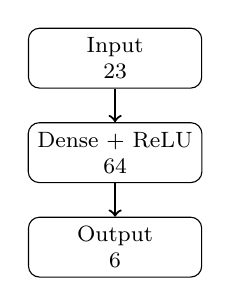
\begin{tikzpicture}[
    node distance=1.2cm,
    every node/.style={draw, rounded corners, minimum width=2.2cm, minimum height=0.7cm, align=center, font=\footnotesize},
    arrow/.style={->, thick}
]
\node (input) {Input\\23};
\node (h1) [below of=input] {Dense + ReLU\\64};
\node (output) [below of=h1] {Output\\6};
\draw[arrow] (input) -- (h1);
\draw[arrow] (h1) -- (output);
\end{tikzpicture}
\caption{Shallow $(64)$}
\end{subfigure}
\hfill
\begin{subfigure}[b]{0.32\textwidth}
\centering
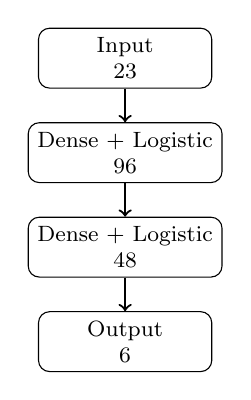
\begin{tikzpicture}[
    node distance=1.2cm,
    every node/.style={draw, rounded corners, minimum width=2.2cm, minimum height=0.7cm, align=center, font=\footnotesize},
    arrow/.style={->, thick}
]
\node (input) {Input\\23};
\node (h1) [below of=input] {Dense + Logistic\\96};
\node (h2) [below of=h1] {Dense + Logistic\\48};
\node (output) [below of=h2] {Output\\6};
\draw[arrow] (input) -- (h1);
\draw[arrow] (h1) -- (h2);
\draw[arrow] (h2) -- (output);
\end{tikzpicture}
\caption{Medium $(96, 48)$}
\end{subfigure}
\hfill
\begin{subfigure}[b]{0.32\textwidth}
\centering
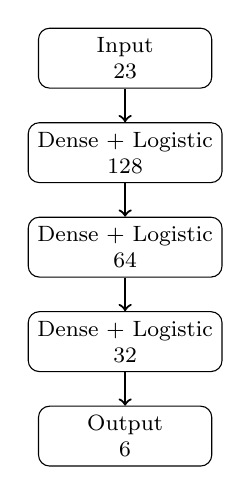
\begin{tikzpicture}[
    node distance=1.2cm,
    every node/.style={draw, rounded corners, minimum width=2.2cm, minimum height=0.7cm, align=center, font=\footnotesize},
    arrow/.style={->, thick}
]
\node (input) {Input\\23};
\node (h1) [below of=input] {Dense + Logistic\\128};
\node (h2) [below of=h1] {Dense + Logistic\\64};
\node (h3) [below of=h2] {Dense + Logistic\\32};
\node (output) [below of=h3] {Output\\6};
\draw[arrow] (input) -- (h1);
\draw[arrow] (h1) -- (h2);
\draw[arrow] (h2) -- (h3);
\draw[arrow] (h3) -- (output);
\end{tikzpicture}
\caption{Deep $(128, 64, 32)$}
\end{subfigure}
\caption{Multilayer perceptron architectures used in the classical benchmark. Each box denotes a fully connected layer followed by the specified activation function. The numbers indicate the layer width (number of neurons). The shallow architecture uses ReLU activation, while the medium and deep architectures use logistic (sigmoid) activation. All three architectures map 23 inputs to 6 measured outputs.}
\label{fig:mlp_architectures}
\end{figure}

The classical regressors produced predictions directly in the measured-output space $\mathbb{R}^K$. Because these models never construct a latent component-space state candidate, there is no physically meaningful basis on which to apply the invariant or non-negativity enforcement developed in Section~2. Consequently, the raw measured-space output of each classical model constitutes its final deployed prediction and is used directly for metric evaluation.

\subsection{Prediction Taxonomy and Metric Definitions}

Before presenting the evaluation protocol, it is necessary to define precisely how the different types of predictions and their associated metrics are distinguished throughout this study.

\subsubsection{Raw and Projected Predictions}

For ICSOR, the term \textit{raw prediction} denotes the measured-space output obtained by collapsing the coupled affine reference prior to constrained deployment, i.e., $y_{raw} = I_{comp}\, c_{aff}$. This reference need not satisfy the exact invariant relation and may imply negative component concentrations. The term \textit{projected prediction} denotes the final reported output $\hat{y}_{ext} = I_{comp}\, \hat{c}$ obtained after the deployment linear program in Eq.~(6) has been solved. The projected prediction is the deployed output of the ICSOR framework.

For the classical regressors, only raw predictions exist. Because these models map inputs directly to measured composites without ever constructing a latent component-space estimate, neither invariant projection nor non-negativity correction can be applied. The raw measured-space output is therefore also the deployed output.

\subsubsection{Effective Metrics}

To enable a fair cross-model comparison, the term \textit{effective prediction} is defined as the deployed output of each model: the projected prediction $\hat{y}_{ext}$ for ICSOR and the raw measured-space prediction $\hat{y}$ for each classical regressor. All cross-model rankings in this study are based exclusively on effective predictions. Correspondingly, the \textit{effective test metric} for a given performance measure (e.g., effective test RMSE) denotes that measure evaluated on the test set using each model's effective prediction, and the \textit{effective training metric} denotes the same measure evaluated on the training set.

\subsubsection{Regression Metrics}

Five standard regression metrics were employed throughout the evaluation, each computed as an aggregate over all $K = 6$ measured output targets. Let $y_i \in \mathbb{R}^K$ and $\hat{y}_i \in \mathbb{R}^K$ denote the observed and predicted measured vectors for sample $i$, respectively, over $N$ evaluation samples with $N_t = N \times K$ total scalar predictions. The metrics are:

\begin{enumerate}
\item \textbf{Coefficient of determination} ($R^2$): Defined as $R^2 = 1 - \sum_{j=1}^{K} \sum_{i=1}^{N} (y_{ij} - \hat{y}_{ij})^2 \Big/ \sum_{j=1}^{K} \sum_{i=1}^{N} (y_{ij} - \bar{y}_j)^2$, where $\bar{y}_j$ is the mean of target $j$ over the evaluation set. Individual per-target $R^2$ scores are averaged uniformly across the $K$ targets.

\item \textbf{Mean squared error} (MSE): $\mathrm{MSE} = \frac{1}{N_t} \sum_{j=1}^{K} \sum_{i=1}^{N} (y_{ij} - \hat{y}_{ij})^2$.

\item \textbf{Root mean squared error} (RMSE): $\mathrm{RMSE} = \sqrt{\mathrm{MSE}}$.

\item \textbf{Mean absolute error} (MAE): $\mathrm{MAE} = \frac{1}{N_t} \sum_{j=1}^{K} \sum_{i=1}^{N} |y_{ij} - \hat{y}_{ij}|$.

\item \textbf{Mean absolute percentage error} (MAPE): $\mathrm{MAPE} = \frac{1}{N_t} \sum_{j=1}^{K} \sum_{i=1}^{N} \frac{|y_{ij} - \hat{y}_{ij}|}{\max(|y_{ij}|,\, \epsilon)}$, with $\epsilon = 10^{-8}$ to guard against division by zero.
\end{enumerate}

These metrics were computed both at the aggregate level (averaging across all targets) and independently for each of the six output targets (COD, TN, TKN, TP, TSS, VSS).

\subsection{Evaluation Protocol}

Each model was trained once on the authoritative 8,000-row training set and evaluated on both the training and test sets. For ICSOR, both raw and projected metrics were recorded so that the impact of the deployment correction could be quantified; however, only the projected (effective) metrics were used for cross-model ranking. For the classical regressors, only raw (effective) metrics were available. Aggregate and per-target regression metrics were computed for all six measured outputs using the five metrics defined above.

Negative-prediction analyses quantified the number and proportion of predicted values below zero, the proportion of samples containing at least one negative prediction, and the minimum negative excursion. ICSOR additionally reported component-space constraint residuals $\|A\hat{c} - Ac_{in}\|$, parity plots in both measured and component spaces, and blockwise visualizations of the learned driver and coupling coefficients.

\subsection{Repeated Dataset-Size Analysis}

To assess sample-efficiency and generalization behavior, each model underwent a repeated dataset-size analysis. The full benchmark dataset was subsampled without replacement at total sizes of 500, 1450, 2400, 3350, 4300, 5250, 6200, 7150, 8100, 9050, and 10,000 rows. Each size was repeated 100 times with distinct but reproducible seeds derived from the base seed 42, and each repeated sample was re-split using the same 20\% test fraction. The resulting analysis therefore comprised 1,100 re-estimated train-test experiments per model. The hyperparameters selected in the main benchmark stage (Table~\ref{tab:optuna_hyperparameters} for classical models; the fixed recursive coupled-QP configuration for ICSOR) were reused throughout this sweep so that the resampling analysis isolated sample-size sensitivity and split variability rather than retuning noise. Performance at each dataset size was summarized by the effective MSE, i.e., the MSE computed from each model's deployed (effective) prediction.

\subsection{Comparative Analysis}

The final cross-model comparison pooled all per-model sweeps into one common evidence bundle. The primary ranking metric was the effective test RMSE, chosen because it remains in the physical measured-output units and penalizes large errors. Supporting summaries included effective test MAE, $R^2$, MAPE, and MSE.

\subsubsection{Normalized Area Under the Learning Curve (NAULC)}

For each model and each metric, the learning curve was constructed by plotting the median effective test metric against training-set size across the 100 repetitions. The area under this curve was computed by trapezoidal integration over the training-size axis. To enable cross-metric comparison, this area was then normalized by dividing by the total span of the training-size axis (i.e., the difference between the maximum and minimum training sizes), yielding the Normalized Area Under the Learning Curve (NAULC). A lower NAULC indicates better sample-averaged performance for error metrics (MSE, RMSE, MAE, MAPE), while a higher NAULC indicates better performance for $R^2$. The NAULC thus provides a single scalar summary of each model's performance integrated across the entire range of available training data, rather than at a single operating point.

\subsubsection{Average Rank}

For each combination of measured output target, performance metric, and training-set size, all models were ranked from best to worst using dense ranking (ties share the same rank). The average rank of a model was then computed as the arithmetic mean of its rank values across all such combinations. This aggregation summarizes how consistently a model performs across heterogeneous evaluation conditions: a low average rank indicates that a model is reliably among the top performers regardless of the specific target, metric, or sample size considered.

\subsubsection{Generalization Gap}

The effective RMSE train-test gap was computed at the largest training size (8,000 training rows) as:
\begin{equation*}
\Delta_{\mathrm{RMSE}} = \overline{\mathrm{RMSE}}_{\mathrm{test}} - \overline{\mathrm{RMSE}}_{\mathrm{train}}
\end{equation*}
where $\overline{\mathrm{RMSE}}_{\mathrm{test}}$ and $\overline{\mathrm{RMSE}}_{\mathrm{train}}$ denote the mean effective RMSE on the test and training sets, respectively, averaged across the 100 resampling repetitions at that size. A positive gap indicates that the model performs worse on unseen data than on training data, with larger gaps suggesting greater overfitting. When expressed as a percentage, the gap is normalized by $\overline{\mathrm{RMSE}}_{\mathrm{train}}$.

\subsubsection{Per-Target Leaderboards}

Per-target effective RMSE leaderboards rank all models independently for each of the six measured outputs (COD, TN, TKN, TP, TSS, VSS). For each target, models are sorted in ascending order of their effective test RMSE at the largest training size, providing a fine-grained view of which model families excel for specific effluent quality indicators.

Physical behavior was assessed in parallel through effective negative-prediction rates and, for ICSOR, the magnitude of raw-to-projected corrections $\|c^* - c_{raw}\|$ and component-space constraint residuals $\|Ac^* - Ac_{in}\|$. These diagnostic quantities were interpreted as complementary descriptors of model behavior rather than as substitute ranking criteria.

\section{Results and Discussion}

This section reports the results of the cross-model comparison described in Section~3. All twelve models---ICSOR, XGBoost, LightGBM, CatBoost, AdaBoost, Random Forest (RF), SVR, $k$-NN, PLS, MLP Shallow, MLP Medium, and MLP Deep---were evaluated under the identical repeated dataset-size analysis protocol. The primary ranking metric is the effective test RMSE, where \textit{effective} denotes the projected prediction $\hat{y}_{ext} = I_{comp}\,\hat{c}$ for ICSOR and the raw measured-space prediction for each classical regressor, as defined in Section~3.6. All results are averaged across the resampling repetitions at each training size unless stated otherwise.

\subsection{Overall Model Ranking at Maximum Training Size}

Table~\ref{tab:leaderboard} presents the effective test metrics for all twelve models at the full training size (8{,}000 samples).

\begin{table}[htbp]
\centering
\caption{Effective test metrics at the full training size (8{,}000 training samples, 2{,}000 test samples), sorted by effective test RMSE rank. ICSOR uses the projected prediction $\hat{y}_{ext} = I_{comp}\,\hat{c}$; all classical models use their raw measured-space output.}
\label{tab:leaderboard}
\small
\begin{tabular}{@{}rlccccc@{}}
\toprule
\textbf{Rank} & \textbf{Model} & \textbf{RMSE} & \textbf{MAE} & \textbf{$R^2$} & \textbf{MAPE} & \textbf{MSE} \\
\midrule
1 & MLP Medium   & 4.887  & 2.305  & 0.9854 & 0.0156 & 23.88 \\
2 & MLP Shallow  & 4.954  & 2.466  & 0.9835 & 0.0172 & 24.54 \\
3 & MLP Deep     & 5.317  & 2.661  & 0.9844 & 0.0175 & 28.27 \\
4 & SVR          & 5.772  & 3.111  & 0.9791 & 0.0223 & 33.32 \\
5 & LightGBM     & 6.500  & 3.681  & 0.9768 & 0.0246 & 42.24 \\
6 & CatBoost     & 6.514  & 3.746  & 0.9742 & 0.0269 & 42.43 \\
7 & XGBoost      & 6.824  & 3.955  & 0.9733 & 0.0270 & 46.56 \\
8 & ICSOR        & 6.942  & 3.929  & 0.9724 & 0.0266 & 48.19 \\
9 & PLS          & 10.348 & 6.271  & 0.9436 & 0.0420 & 107.09 \\
10 & AdaBoost    & 15.151 & 9.867  & 0.8815 & 0.0726 & 229.56 \\
11 & RF          & 16.266 & 10.036 & 0.8806 & 0.0693 & 264.58 \\
12 & $k$-NN      & 18.166 & 11.913 & 0.7956 & 0.0941 & 330.00 \\
\bottomrule
\end{tabular}
\end{table}

Three distinct performance tiers emerge. The \textbf{top tier} consists of the three MLP architectures and SVR, which separate decisively from all other models. MLP Medium achieves the lowest effective test RMSE (4.887), closely followed by MLP Shallow (4.954) and MLP Deep (5.317). Notably, the Optuna-selected activation functions differ across the three MLP variants: the shallow network uses ReLU, while the medium and deep networks use logistic (sigmoid) activation. Despite this difference, MLP Medium retains the top position. SVR, equipped with an Optuna-optimized degree-4 polynomial kernel, achieves a RMSE of 5.772, closing much of the gap to the MLP tier. The top four models explain 97.9--98.5\% of the effluent variance ($R^2 \ge 0.979$), and their MAPE values of 1.6--2.2\% indicate that the mean prediction error remains below 2.5\% of the effluent magnitude. An interesting rank inversion occurs between MLP Shallow and MLP Deep: while MLP Shallow achieves the lower RMSE (4.954 vs.\ 5.317), MLP Deep achieves the higher $R^2$ (0.9844 vs.\ 0.9835). This indicates that MLP Deep distributes its errors more uniformly across the target range, whereas MLP Shallow achieves a marginally lower total squared error at the cost of slightly less balanced relative accuracy.

The \textbf{middle tier} spans LightGBM (6.500), CatBoost (6.514), XGBoost (6.824), and ICSOR (6.942), a range of only 0.44~RMSE units. ICSOR achieves the lowest MAE in this group (3.929), which is lower than XGBoost (3.955) and comparable to CatBoost (3.746) and LightGBM (3.681), despite ranking 8th in RMSE. This indicates that ICSOR's error distribution has lighter tails relative to its squared-error magnitude, consistent with the regularizing effect of the invariant projection $c^* \in \mathcal{S}_+(c_{in})$ developed in Section~2.4. The $R^2$ values of the middle tier range from 0.9724 (ICSOR) to 0.9768 (LightGBM), confirming that all four models explain over 97\% of the test-set variance.

The \textbf{bottom tier} includes PLS (10.348), AdaBoost (15.151), RF (16.266), and $k$-NN (18.166). These models deliver effective test RMSE values 2--4$\times$ worse than the top tier. The particularly poor performance of $k$-NN ($R^2 = 0.796$, MAPE $= 9.4\%$) renders it unsuitable for this prediction task. PLS, while achieving a respectable $R^2$ (0.944), is fundamentally limited by its inability to capture the Monod-type multiplicative nonlinearities in the ASM2d-TSN kinetics using its linear latent-variable structure.

\subsection{Consistency Across Metrics and Training Sizes: Average Rank Analysis}

Table~\ref{tab:leaderboard} ranks models at the full training size. To assess consistency across a broader range of data availability, the average rank of each model was computed across all training sizes (400--8{,}000), all six measured output targets, and all five metrics, as defined in Section~3.7.2. The results are presented in Fig.~\ref{fig:lc_rmse_mae} and Fig.~\ref{fig:lc_r2_mape}, which depict the effective test learning curves. The average rank heatmap is shown in Fig.~\ref{fig:avg_rank_heatmap}.

\begin{figure}[htbp]
\centering

\includegraphics[width=0.85\textwidth]{placeholder.png}
\caption{Average rank heatmap across all training sizes, measured output targets, and metrics. Lower average rank (darker shading) indicates more consistent top performance across the full evaluation protocol.}
\label{fig:avg_rank_heatmap}
\end{figure}

The average rank analysis confirms the MLP tier's dominance. MLP Medium retains the top position, while the ordering between MLP Shallow and MLP Deep is sensitive to the range of training sizes considered. At large data sizes, the deeper architecture benefits from its additional capacity, whereas at smaller sizes the shallower architecture's lower variance yields better sample-averaged performance, consistent with the classical bias-variance tradeoff.

The most notable finding concerns ICSOR. While ICSOR ranks 8th at the full training size (Table~\ref{tab:leaderboard}), the learning curves show that it is more competitive at smaller training sizes, where unconstrained regressors suffer from higher variance. This reflects the inductive bias provided by the stoichiometric constraint projection $c^* \in \mathcal{S}_+(c_{in})$, which restricts the effective hypothesis space and performs implicit regularization. At small training sizes where unconstrained regressors have high variance, ICSOR's physics-informed structure compensates for the limited data, yielding lower effective errors than most classical alternatives.

\subsection{Sample Efficiency: Learning Curve Analysis}

Figure~\ref{fig:lc_rmse_mae} presents the effective test RMSE and MAE learning curves across all training sizes. Figure~\ref{fig:lc_r2_mape} presents the corresponding $R^2$ and MAPE learning curves. The shaded bands represent the interquartile range across the resampling repetitions.

\begin{figure}[htbp]
\centering
\begin{subfigure}[b]{0.48\textwidth}
\centering
% Placeholder: RMSE learning curve
% Path: results/plot_results/comparison/plots/effective_rmse_learning_curve_20260407_165106.png

\includegraphics[width=\textwidth]{placeholder.png}
\caption{Effective test RMSE}
\end{subfigure}
\hfill
\begin{subfigure}[b]{0.48\textwidth}
\centering
% Placeholder: MAE learning curve
% Path: results/plot_results/comparison/plots/effective_mae_learning_curve_20260407_165106.png

\includegraphics[width=\textwidth]{placeholder.png}
\caption{Effective test MAE}
\end{subfigure}
\caption{Effective test RMSE and MAE learning curves across training sizes (400--8{,}000 samples). Lines denote the mean across resampling repetitions; shaded bands represent the interquartile range. All twelve models share identical train-test partitions at each size.}
\label{fig:lc_rmse_mae}
\end{figure}

\begin{figure}[htbp]
\centering
\begin{subfigure}[b]{0.48\textwidth}
\centering
% Placeholder: R2 learning curve
% Path: results/plot_results/comparison/plots/effective_r2_learning_curve_20260407_165106.png

\includegraphics[width=\textwidth]{placeholder.png}
\caption{Effective test $R^2$}
\end{subfigure}
\hfill
\begin{subfigure}[b]{0.48\textwidth}
\centering
% Placeholder: MAPE learning curve
% Path: results/plot_results/comparison/plots/effective_mape_learning_curve_20260407_165106.png

\includegraphics[width=\textwidth]{placeholder.png}
\caption{Effective test MAPE}
\end{subfigure}
\caption{Effective test $R^2$ and MAPE learning curves across training sizes (400--8{,}000 samples). Higher $R^2$ is better; lower MAPE is better.}
\label{fig:lc_r2_mape}
\end{figure}

The learning curves in Fig.~\ref{fig:lc_rmse_mae} exhibit three visually distinct trajectory groups. The MLP and SVR curves descend steeply, crossing below the middle tier before approximately 1{,}200 training samples. The middle-tier models (ICSOR, LightGBM, XGBoost, CatBoost) follow a shallower descent. The bottom-tier models (PLS, RF, AdaBoost, $k$-NN) show either very slow improvement or persistently high error.

Table~\ref{tab:naulc} quantifies these trajectories through the Normalized Area Under the Learning Curve (NAULC) defined in Section~3.7.1. For error metrics (RMSE, MAE, MAPE, MSE), a lower NAULC indicates better sample-averaged performance; for $R^2$, a higher NAULC is better.

\begin{table}[htbp]
\centering
\caption{Normalized Area Under the Learning Curve (NAULC) for each model and metric, computed by trapezoidal integration of the effective test metric over the training-size axis and normalized by the training-size span. For RMSE, MAE, MAPE, and MSE, lower is better; for $R^2$, higher is better. Models are sorted by RMSE NAULC.}
\label{tab:naulc}
\small
\begin{tabular}{@{}rlccccc@{}}
\toprule
\textbf{Rank} & \textbf{Model} & \textbf{RMSE} & \textbf{MAE} & \textbf{$R^2$} & \textbf{MAPE} & \textbf{MSE} \\
\midrule
1  & MLP Medium   & 6.350 & 3.465 & 0.9733 & 0.0251 & 43.58  \\
2  & MLP Shallow  & 6.562 & 3.655 & 0.9727 & 0.0260 & 45.85  \\
3  & MLP Deep     & 6.663 & 3.684 & 0.9712 & 0.0262 & 48.33  \\
4  & ICSOR        & 8.117 & 4.577 & 0.9639 & 0.0296 & 73.24  \\
5  & LightGBM     & 8.369 & 4.807 & 0.9655 & 0.0307 & 72.88  \\
6  & SVR          & 8.832 & 5.171 & 0.9565 & 0.0370 & 80.61  \\
7  & XGBoost      & 8.893 & 5.109 & 0.9614 & 0.0328 & 82.66  \\
8  & CatBoost     & 8.983 & 5.284 & 0.9566 & 0.0370 & 83.63  \\
9  & PLS          & 14.336 & 8.855 & 0.9120 & 0.0554 & 205.77 \\
10 & RF           & 18.715 & 11.521 & 0.8466 & 0.0783 & 352.30 \\
11 & AdaBoost     & 21.462 & 13.282 & 0.8186 & 0.0859 & 461.02 \\
12 & $k$-NN       & 21.854 & 14.075 & 0.7332 & 0.1042 & 478.99 \\
\bottomrule
\end{tabular}
\end{table}

The NAULC confirms the impressions from the learning curves. Within the MLP tier, MLP Medium achieves the best NAULC on all five metrics, and MLP Shallow outperforms MLP Deep (RMSE NAULC 6.562 vs.\ 6.663). This confirms that the deeper MLP architecture's advantage materializes principally at larger training sizes; when performance is integrated across the full data regime, the shallower architecture with fewer parameters is more sample-efficient.

ICSOR achieves the 4th-best RMSE NAULC (8.117), placing it ahead of the gradient-boosted tree and ensemble regressors. Compared to LightGBM (8.369), ICSOR's 3.0\% NAULC advantage reflects the physics-informed inductive bias discussed in Section~2: the stoichiometric constraint projection $c^* \in \mathcal{S}_+(c_{in})$ reduces the effective dimensionality of the hypothesis space, so that the model achieves competitive accuracy with fewer training samples. This advantage is most pronounced at the smallest training sizes (Fig.~\ref{fig:lc_rmse_mae}a), where the unconstrained regressors suffer from higher variance. As training data grows and the unconstrained models converge, ICSOR's advantage narrows, and at 8{,}000 samples it is surpassed by SVR, LightGBM, CatBoost, and XGBoost in point-wise RMSE (Table~\ref{tab:leaderboard}).

The $R^2$ NAULC further illustrates the separation between tiers. The MLP models sustain $R^2 > 0.97$ on average across the full sweep, while the middle-tier models achieve $R^2 = 0.956$--$0.966$. ICSOR's $R^2$ NAULC (0.9639) is slightly below LightGBM's (0.9655) but well above CatBoost (0.9566) and SVR (0.9565). The bottom-tier models fall below $R^2 = 0.91$ on average, with $k$-NN explaining only 73.3\% of the output variance across the full training-size range---unacceptable for most practical applications.

\subsection{Per-Target Performance Analysis}

Table~\ref{tab:per_target} reports the effective test RMSE for each model at the full training size, disaggregated by the six measured output targets $y = I_{comp}\,c_{out}$: COD, TN, TKN, TP, TSS, and VSS. The per-target effective RMSE heatmap is presented in Fig.~\ref{fig:target_heatmaps}a.

\begin{table}[htbp]
\centering
\caption{Effective test RMSE by measured output target at the full training size (8{,}000 training samples). Bold denotes the best model for each target. Models are sorted by overall effective test RMSE rank (Table~\ref{tab:leaderboard}).}
\label{tab:per_target}
\small
\begin{tabular}{@{}rlcccccc@{}}
\toprule
\textbf{Rank} & \textbf{Model} & \textbf{COD} & \textbf{TN} & \textbf{TKN} & \textbf{TP} & \textbf{TSS} & \textbf{VSS} \\
\midrule
1 & MLP Medium   & 7.647  & \textbf{1.047}  & 3.030  & 0.473  & \textbf{6.434}  & \textbf{5.737} \\
2 & MLP Shallow  & \textbf{7.174}  & 1.109  & 3.350  & 0.430  & 6.768  & 6.110 \\
3 & MLP Deep     & 8.270  & 1.171  & \textbf{2.899}  & 0.475  & 7.270  & 6.193 \\
4 & SVR          & 8.638  & 1.594  & 3.497  & 0.453  & 7.747  & 7.092 \\
5 & LightGBM     & 10.597 & 1.685  & 3.498  & 0.470  & 8.234  & 7.620 \\
6 & CatBoost     & 10.191 & 1.798  & 3.827  & 0.563  & 8.604  & 7.648 \\
7 & XGBoost      & 11.106 & 1.742  & 3.915  & 0.484  & 8.701  & 7.856 \\
8 & ICSOR        & 10.993 & 1.646  & 4.060  & \textbf{0.396}  & 8.922  & 8.326 \\
9 & PLS          & 16.947 & 1.996  & 5.803  & 0.490  & 13.360 & 11.788 \\
10 & AdaBoost    & 27.406 & 2.821  & 8.273  & 1.449  & 17.011 & 16.076 \\
11 & RF          & 31.979 & 3.985  & 6.188  & 2.328  & 16.419 & 15.350 \\
12 & $k$-NN      & 32.922 & 6.527  & 8.125  & 3.410  & 20.201 & 19.177 \\
\bottomrule
\end{tabular}
\end{table}

\begin{figure}[htbp]
\centering
\begin{subfigure}[b]{0.48\textwidth}
\centering
% Placeholder: Per-target RMSE heatmap
% Path: results/plot_results/comparison/plots/effective_rmse_by_target_heatmap_20260407_165106.png

\includegraphics[width=\textwidth]{placeholder.png}
\caption{Effective RMSE by target}
\end{subfigure}
\hfill
\begin{subfigure}[b]{0.48\textwidth}
\centering
% Placeholder: Per-target negative rate heatmap
% Path: results/plot_results/comparison/plots/negative_prediction_rate_by_target_heatmap_20260407_165106.png

\includegraphics[width=\textwidth]{placeholder.png}
\caption{Negative prediction rate by target}
\end{subfigure}
\caption{Per-target diagnostic heatmaps at the largest training size (8{,}000 samples). (a)~Effective test RMSE for each model and measured output target. (b)~Percentage of predicted values below zero for each model and target. Models are ordered by overall average rank (best at top).}
\label{fig:target_heatmaps}
\end{figure}

The per-target analysis reveals that the aggregate ranking conceals a physically meaningful exception. \textbf{ICSOR achieves the best RMSE on total phosphorus (TP)}: 0.396, surpassing all three MLP architectures (MLP Shallow: 0.430, SVR: 0.453, LightGBM: 0.470, MLP Medium: 0.473, MLP Deep: 0.475). This is the only target on which ICSOR ranks 1st, and the result has a clear mechanistic interpretation. In the ASM2d-TSN framework, total phosphorus is tightly governed by the stoichiometric constraints associated with phosphorus-accumulating organisms ($X_{PAO}$), the polyphosphate pool ($X_{PP}$), and the metal precipitation pathways ($X_{MeP}$). The invariant projection $Ac^* = Ac_{in}$ enforced by ICSOR (Eq.~2) directly preserves the conserved phosphorus balance implied by the left null space of $\nu$. This hard constraint reduces the effective degrees of freedom available to the prediction, funneling the model toward the physically correct solution along the phosphorus-balance manifold. The MLP models, which predict directly in the measured output space $\mathbb{R}^K$ without access to the latent component-space structure, must learn this balance implicitly from data. At 8{,}000 samples, their implicit learning of the phosphorus balance falls short of the guarantee provided by the explicit projection.

For \textbf{COD}, which represents the broadest aggregate of organic and biomass fractions, MLP Shallow leads (7.174) and ICSOR ranks 7th (10.993). The 53\% relative increase in ICSOR's COD error compared to MLP Shallow reflects the fact that COD dynamics are predominantly governed by the total magnitude and general nonlinear patterns of the input-output mapping rather than by specific stoichiometric detail. The second-order feature map $\phi(u, c_{in})$ used by ICSOR (Eq.~3) captures pairwise interactions but cannot represent the higher-order nonlinearities that the MLP architectures approximate through their hidden layers.

For \textbf{TKN} (Total Kjeldahl Nitrogen), MLP Deep is the best (2.899), followed by MLP Medium (3.030) and MLP Shallow (3.350). SVR (3.497) and LightGBM (3.498) also outperform ICSOR (4.060), indicating that for nitrogen species, the models with higher approximation capacity capture the relevant input-output structure more effectively than ICSOR's constrained quadratic framework.

For \textbf{TN} (Total Nitrogen), MLP Medium leads (1.047), followed by MLP Shallow (1.109) and MLP Deep (1.171). ICSOR ranks 5th (1.646). The small absolute magnitudes reflect the narrow dynamic range of total nitrogen in the ASM2d-TSN simulation domain.

For \textbf{TSS and VSS} (Total and Volatile Suspended Solids), the ranking pattern is nearly identical for both targets, as expected from the linear relationship $\text{VSS} \subset \text{TSS}$ encoded in $I_{comp}$. MLP Medium (TSS: 6.434, VSS: 5.737) leads on both targets. ICSOR ranks 8th on both targets (TSS: 8.922, VSS: 8.326), behind the gradient-boosted tree models and SVR. The solids targets are influenced by biomass growth fractions, processes whose nonlinearity exceeds the capacity of the second-order feature map, placing ICSOR at a structural disadvantage for these outputs.

In summary, the per-target analysis delineates a clear pattern: ICSOR's stoichiometric constraint projection provides the greatest advantage on targets most tightly coupled to the conserved quantities of the ASM2d-TSN reaction network (TP), provides moderate benefit for nitrogen-balance targets (TN, TKN), and confers no advantage for the empirical aggregate targets (COD, TSS, VSS), where the unconstrained models with higher approximation capacity dominate.

\subsection{Generalization Gap Analysis}

Table~\ref{tab:gen_gap} reports the effective RMSE generalization gap $\Delta_{\mathrm{RMSE}}$ at the full training size, as defined in Section~3.7.3.

\begin{table}[htbp]
\centering
\caption{Effective RMSE generalization gap at the full training size (8{,}000 training samples). The gap is defined as $\Delta_{\mathrm{RMSE}} = \mathrm{RMSE}_{\mathrm{test}} - \mathrm{RMSE}_{\mathrm{train}}$. The percentage is normalized by $\mathrm{RMSE}_{\mathrm{train}}$. Models are sorted by gap percentage.}
\label{tab:gen_gap}
\small
\begin{tabular}{@{}rlcccc@{}}
\toprule
& \textbf{Model} & $\mathrm{RMSE}_{\mathrm{test}}$ & $\mathrm{RMSE}_{\mathrm{train}}$ & $\Delta_{\mathrm{RMSE}}$ & \textbf{Gap \%} \\
\midrule
& PLS          & 10.348 & 10.554 & $-$0.206 & $-$2.0\% \\
& AdaBoost     & 15.151 & 15.050 & 0.101  & 0.7\%   \\
& ICSOR        & 6.942  & 6.770  & 0.172  & 2.5\%   \\
& MLP Deep     & 5.317  & 4.474  & 0.843  & 18.8\%  \\
& CatBoost     & 6.514  & 5.228  & 1.286  & 24.6\%  \\
& MLP Shallow  & 4.954  & 3.974  & 0.980  & 24.7\%  \\
& XGBoost      & 6.824  & 4.959  & 1.865  & 37.6\%  \\
& SVR          & 5.772  & 3.697  & 2.075  & 56.1\%  \\
& LightGBM     & 6.500  & 3.731  & 2.769  & 74.2\%  \\
& MLP Medium   & 4.887  & 2.782  & 2.105  & 75.7\%  \\
& RF           & 16.266 & 3.249  & 13.017 & 400.6\% \\
& $k$-NN       & 18.166 & $\approx$0 & 18.166 & $>$10$^{9}$\% \\
\bottomrule
\end{tabular}
\end{table}

\begin{figure}[htbp]
\centering
% Placeholder: Generalization gap learning curve
% Path: results/plot_results/comparison/plots/effective_rmse_generalization_gap_20260407_165106.png

\includegraphics[width=0.85\textwidth]{placeholder.png}
\caption{Effective RMSE generalization gap ($\Delta_{\mathrm{RMSE}} = \overline{\mathrm{RMSE}}_{\mathrm{test}} - \overline{\mathrm{RMSE}}_{\mathrm{train}}$) as a function of training size. Smaller gaps indicate better generalization. ICSOR (bold) maintains one of the smallest gaps across all training sizes.}
\label{fig:gen_gap}
\end{figure}

The generalization gap analysis reveals a striking dichotomy between predictive accuracy and overfitting behavior. Among competitive models (effective test RMSE $< 10$), \textbf{ICSOR exhibits the smallest positive generalization gap} at 2.5\%, meaning its training-set performance is nearly identical to its test-set performance. This is a direct consequence of the physics-informed constraint structure: the projection $c^* \in \mathcal{S}_+(c_{in})$ restricts the effective model capacity by confining predictions to the invariant-consistent non-negative set, thereby acting as a structural regularizer in the same spirit as the $P_{adm}$ projection (Eq.~7). PLS achieves a slightly negative gap ($-2.0\%$), indicating marginal underfitting rather than genuine generalization superiority---the model is too constrained to fit the data fully. AdaBoost shows a small positive gap (0.7\%) but its high absolute error (15.15~RMSE) similarly indicates chronic underfitting.

The top-performing MLP models exhibit heterogeneous gap behavior. MLP Deep achieves a moderate gap (18.8\%), while MLP Shallow shows a gap of 24.7\%. MLP Medium, despite achieving the best test RMSE, exhibits a gap of 75.7\%, indicating that it memorizes a considerable fraction of training patterns (train RMSE 2.78 vs.\ test RMSE 4.89). However, its absolute test error remains the best of all models, confirming that the overfitting has not yet degraded generalization to the point where less flexible models are preferable. SVR shows a gap of 56.1\%, reflecting its flexible polynomial kernel mapping, while LightGBM reaches 74.2\%.

The tree-based ensemble methods show variable gaps. CatBoost (24.6\%) and XGBoost (37.6\%) are moderate, while RF (400.6\%) achieves low training error through deep tree structures but pays a severe generalization penalty. $k$-NN achieves near-zero training error by construction (it memorizes the training points exactly) but produces the highest test error of all models, confirming that nearest-neighbor interpolation fails in this high-dimensional, nonlinear problem.

\textbf{ICSOR's generalization gap is therefore the best among all models with competitive absolute performance.} This property has practical importance for reliable deployment: if the deployment data distribution shifts modestly from the training distribution, ICSOR's predictions are the least likely to degrade among the set of middle-tier and upper-tier models. The gap remains small across the full training-size sweep (Fig.~\ref{fig:gen_gap}), indicating that this conclusion is not specific to the full training size.

\subsection{Physical Plausibility Diagnostics}

\subsubsection{Negative Prediction Rates}

At the full training size, the one-shot benchmark summaries still report zero negative predictions on the test set for all twelve models, including PLS. However, the repeated dataset-size sweep underlying Fig.~\ref{fig:target_heatmaps}b resolves a vanishing residual PLS signal at the largest training size: the diagnostic summary gives a mean negative-prediction rate of 0.0008\% with standard deviation 0.0026\%, whereas every other model remains at exactly 0.0\%. The heatmap is therefore still visually dominated by zeros, but it no longer supports the stronger claim of uniform exact zeros for every model across the repeated splits.

However, this near-absence of negatives carries a fundamentally different epistemological status for ICSOR than for the classical regressors. For ICSOR, zero negatives is guaranteed by construction: the linear program in Eq.~(6) enforces $\hat{c} \ge 0$ in the latent component space, and the entrywise non-negativity of the relevant rows of $I_{comp}$ then ensures $\hat{y}_{ext} = I_{comp}\,\hat{c} \ge 0$ in the measured output space. For the remaining models, the near-zero negative rate is still a data-dependent observation that could change under different input distributions, smaller training sets, or extrapolation beyond the simulation domain.

\subsubsection{Raw-to-Projected Correction Magnitude}

Figure~\ref{fig:icsor_diagnostics}a shows the raw-to-projected correction magnitude $\|c^* - c_{raw}\|_2$ for ICSOR across training sizes. This quantity measures how much the stoichiometric invariant projection and non-negativity correction (Section~2.4) alter the unconstrained second-order surrogate prediction before it is collapsed to the measured output.

\begin{figure}[htbp]
\centering
\begin{subfigure}[b]{0.48\textwidth}
\centering
% Placeholder: Raw-to-effective adjustment learning curve
% Path: results/plot_results/comparison/plots/raw_to_effective_adjustment_learning_curve_20260407_165106.png

\includegraphics[width=\textwidth]{placeholder.png}
\caption{Raw-to-projected adjustment $\|c^* - c_{raw}\|_2$}
\end{subfigure}
\hfill
\begin{subfigure}[b]{0.48\textwidth}
\centering
% Placeholder: Constraint residual learning curve
% Path: results/plot_results/comparison/plots/effective_constraint_residual_learning_curve_20260407_165106.png

\includegraphics[width=\textwidth]{placeholder.png}
\caption{Constraint residual $\|Ac^* - Ac_{in}\|_2$}
\end{subfigure}
\caption{ICSOR-specific physical diagnostics across training sizes. (a)~L2 norm of the correction applied by the stoichiometric invariant projection and non-negativity quadratic program. The decreasing trend indicates that the raw surrogate $c_{raw} = \widehat{B}_{ls}\,\phi(u,c_{in})$ progressively aligns with the physical constraint structure as training data grows. (b)~L2 norm of the constraint residual $Ac^* - Ac_{in}$, confirming machine-precision satisfaction of the stoichiometric invariant at all training sizes.}
\label{fig:icsor_diagnostics}
\end{figure}

The correction magnitude begins at approximately 80.0 at 400 training samples and decreases monotonically to 69.9 at 8{,}000 samples, a 12.6\% reduction. This trend has a clear interpretation within the ICSOR framework developed in Section~2. As the training set grows, the least-squares estimate of the affine core, $\widehat{M}^T = \Phi^+\left(Y - C_{in} H^T\right)$ (Section~2.6), becomes more accurate, and the induced latent representative $\widehat{B}_{ls} = G^+\widehat{M}$ yields raw component-space predictions $c_{raw}$ that are increasingly consistent with the stoichiometric invariants. The projection $c_{aff} = P_{adm}\,c_{raw} + P_{inv}\,c_{in}$ therefore needs to correct a progressively smaller deviation, reflected in the decreasing $\|c^* - c_{raw}\|_2$.

Equally important, the standard deviation of the correction magnitude decreases from 7.55 at 400 samples to 0.23 at 8{,}000 samples---a 97\% reduction in variability. This stabilization indicates that ICSOR's raw predictions become highly consistent at large data sizes, requiring a nearly constant correction. This is a desirable operational property: the model's behavior becomes predictable, and the stoichiometric projection acts as a stable, deterministic post-processing layer rather than a stochastic rescue mechanism.

\subsubsection{Constraint Satisfaction Residuals}

Figure~\ref{fig:icsor_diagnostics}b shows the L2 norm of the constraint residual $\|Ac^* - Ac_{in}\|_2$ for ICSOR across training sizes. This residual quantifies how closely the final projected prediction satisfies the stoichiometric invariant $Ac = Ac_{in}$ derived in Section~2.2. The residual is on the order of $5 \times 10^{-11}$ across all training sizes, ranging from $6.3 \times 10^{-11}$ at 400 samples to $4.9 \times 10^{-11}$ at 8{,}000 samples. This is essentially machine-precision satisfaction, confirming that the OSQP solver reliably enforces the conservation law $Ac^* = Ac_{in}$ to numerical precision regardless of the quality of the raw prediction $c_{raw}$ or the training-set size. The invariants of the ASM2d-TSN reaction network are therefore preserved in every ICSOR prediction by construction, a guarantee that no classical regressor can provide.

\subsection{Interpretability of the ICSOR Affine Core}

Unlike the classical benchmark models, ICSOR exposes an interpretable measured-space affine core through the identifiable block matrix
\begin{equation*}
M = \begin{bmatrix}
b_y & W_{u,y} & W_{in,y} \\
\Theta_{uu,y} & \Theta_{cc,y} & \Theta_{uc,y}
\end{bmatrix},
\end{equation*}
introduced in Section~2.5. Because $M$ is identified directly from measured data whereas the latent representative $B$ is not (Section~2.6), the coefficient plots are the most defensible engineering summary of how the surrogate organizes operating effects, influent carry-through, and second-order interactions. These plots must be interpreted carefully: they describe the affine core $y_{aff} = M\phi(u,c_{in}) + Hc_{in}$ before the sample-specific positivity correction $\delta_+$ is applied. They therefore encode signed structural tendencies of the learned surrogate rather than global partial derivatives of the fully corrected deployed prediction $y^*$.

Table~\ref{tab:icsor_density} turns the qualitative sparsity visible in the coefficient plots into a quantitative regularization diagnostic. For each output equation $y$, a coefficient is counted as retained when its absolute value satisfies $|\beta| \ge 0.001 \max_{\beta' \in \mathcal{E}_y} |\beta'|$, where $\mathcal{E}_y$ denotes the full identifiable coefficient set for that target equation. This equation-adaptive rule is preferable to a single global cutoff because the six output equations live on materially different numerical scales; in the present fit it induces absolute thresholds ranging from $5.1 \times 10^{-4}$ to $5.4 \times 10^{-2}$. Under this criterion, 570 of the 3{,}066 coefficients in the identifiable affine core are retained. The first-order terms are therefore largely preserved, but the highest-dimensional interaction block remains sparse: $\Theta_{cc,y}$ retains only 305 of 2{,}646 influent-influent interaction coefficients (11.5\%). This indicates meaningful implicit regularization because the fitted surrogate continues to avoid a dense use of the quadratic basis.

\begin{table}[htbp]
\centering
\caption{ICSOR coefficient density analysis for the identifiable affine core $M$. A coefficient in target equation $y$ is counted as retained when $|\beta| \ge 0.001 \max_{\beta' \in \mathcal{E}_y} |\beta'|$, so the threshold adapts to the native scale of each target equation.}
\label{tab:icsor_density}
\small
\begin{tabular}{@{}lrrr@{}}
\toprule
\textbf{Block} & \textbf{Candidates} & \textbf{Retained} & \textbf{Retention (\%)} \\
\midrule
$b_y$ & 6 & 6 & 100.0 \\
$W_{u,y}$ & 12 & 12 & 100.0 \\
$W_{in,y}$ & 126 & 114 & 90.5 \\
$\Theta_{uu,y}$ & 24 & 20 & 83.3 \\
$\Theta_{uc,y}$ & 252 & 113 & 44.8 \\
$\Theta_{cc,y}$ & 2646 & 305 & 11.5 \\
\midrule
Total & 3066 & 570 & 18.6 \\
\bottomrule
\end{tabular}
\end{table}

\begin{figure}[htbp]
\centering
\begin{subfigure}[b]{0.32\textwidth}
\centering
% Placeholder: ICSOR operational coefficient heatmap
% Path: results/plot_results/training/icsor/coefficients/w_u_heatmap_20260407_060250.png

\includegraphics[width=\textwidth]{placeholder.png}
\caption{$W_{u,y}$}
\end{subfigure}
\hfill
\begin{subfigure}[b]{0.32\textwidth}
\centering
% Placeholder: ICSOR influent coefficient heatmap
% Path: results/plot_results/training/icsor/coefficients/w_in_heatmap_20260407_060250.png

\includegraphics[width=\textwidth]{placeholder.png}
\caption{$W_{in,y} + H$}
\end{subfigure}
\hfill
\begin{subfigure}[b]{0.32\textwidth}
\centering
% Placeholder: ICSOR bias bar chart
% Path: results/plot_results/training/icsor/coefficients/bias_bar_chart_20260407_060250.png

\includegraphics[width=\textwidth]{placeholder.png}
\caption{$b_y$}
\end{subfigure}
\caption{First-order coefficient plots of the identifiable ICSOR affine core in measured space. The displayed quantities correspond to the ICSOR blocks defined in Section~2.5.}
\label{fig:icsor_coeff_first_order}
\end{figure}

\begin{figure}[htbp]
\centering
\begin{subfigure}[b]{0.32\textwidth}
\centering
% Placeholder: ICSOR operational interaction tensor heatmaps
% Path: results/plot_results/training/icsor/coefficients/theta_uu_heatmaps_20260407_060250.png

\includegraphics[width=\textwidth]{placeholder.png}
\caption{$\Theta_{uu,y}$}
\end{subfigure}
\hfill
\begin{subfigure}[b]{0.32\textwidth}
\centering
% Placeholder: ICSOR operational-influent interaction tensor heatmaps
% Path: results/plot_results/training/icsor/coefficients/theta_uc_heatmaps_20260407_060250.png

\includegraphics[width=\textwidth]{placeholder.png}
\caption{$\Theta_{uc,y}$}
\end{subfigure}
\hfill
\begin{subfigure}[b]{0.32\textwidth}
\centering
% Placeholder: ICSOR influent interaction tensor heatmaps
% Path: results/plot_results/training/icsor/coefficients/theta_cc_heatmaps_20260407_060250.png

\includegraphics[width=\textwidth]{placeholder.png}
\caption{$\Theta_{cc,y}$}
\end{subfigure}
\caption{Second-order coefficient plots of the identifiable ICSOR affine core in measured space. These plots separate pure operating curvature, mixed operating-influent interactions, and pure influent interactions, enabling a direct engineering reading of the model structure developed in Section~2.}
\label{fig:icsor_coeff_second_order}
\end{figure}

Figure~\ref{fig:icsor_coeff_first_order} shows that the intercept and the first-order blocks already recover an interpretable engineering story. The bias vector $b_y$ is dominated by COD, with smaller positive baseline contributions for VSS, TSS, and TN, a negative offset for TKN, and an approximately zero offset for TP. This means that, in the affine core alone, the model is anchored primarily by organic-load and solids-related baseline structure, whereas phosphorus is explained much less by a free intercept and much more by influent-dependent and invariant-driven terms.

The operating block $W_{u,y}$ reveals that aeration is the dominant first-order operational lever in measured space. HRT coefficients are weak for nearly every measured output except COD, whereas the aeration column carries the strongest signed structure: a pronounced negative association with COD, a smaller negative association with VSS, modest positive contributions to TKN and TSS, and near-zero first-order influence on TP. This matches the process interpretation of the reactor: changes in oxygen supply directly redistribute oxidation and biomass-related responses, whereas HRT enters more weakly at first order and appears mainly through interaction structure.

The combined influent block $W_{in,y} + H$ is structured and sparse rather than diffuse. COD and the solids outputs draw from a broader set of influent channels, while the TP row is concentrated on a smaller phosphorus-relevant subset. The most prominent columns are associated with dissolved oxygen and nutrient-bearing fractions, confirming that the invariant carry-through term $Hc_{in}$ and the learned linear correction $W_{in,y}c_{in}$ work together to preserve a physically organized dependence on influent composition rather than spreading weight indiscriminately across all 21 ASM2d-TSN influent states.

Figure~\ref{fig:icsor_coeff_second_order} further clarifies where ICSOR locates nonlinearity. In $\Theta_{uu,y}$, the dominant curvature is concentrated almost entirely in the aeration-aeration entry. The HRT-HRT and HRT$\times$Aeration terms are nearly negligible across all outputs, whereas the aeration-squared term is strongly positive for COD and TKN, strongly negative for TSS and VSS, and close to zero for TP. Thus, the principal nonlinear operating behavior learned by ICSOR is not generic curvature in all process levers, but a specific curvature in the oxygen-supply direction.

The mixed block $\Theta_{uc,y}$ shows that aeration does not act independently of the incoming material inventory. Across COD, TN, TKN, TSS, and VSS, the aeration row contains the dominant interaction pattern, while the HRT row remains comparatively flat. COD exhibits the richest mixed structure, with alternating positive and negative hotspots across soluble and particulate influent fractions, indicating that the effectiveness of aeration depends strongly on the entering ASM2d-TSN composition. By contrast, the TP panel is nearly blank, reinforcing the earlier conclusion from Table~\ref{tab:per_target}: phosphorus prediction in ICSOR is governed primarily by invariant-preserving low-order structure rather than by diffuse operating-influent interactions.

Finally, the influent-influent block $\Theta_{cc,y}$ is highly sparse. Most of its entries are near zero, with only a small number of localized hotspots centered on dissolved oxygen and selected nitrogen- and phosphorus-bearing channels. This sparsity is itself an interpretability result. Although ICSOR permits the full second-order term $c_{in} \otimes c_{in}$, the identified affine core does not distribute weight densely across all 441 possible pairs. Instead, it isolates a limited set of nonlinear state couplings that materially influence each measured output. This makes the model auditable: a process engineer can inspect a small subset of coefficient hotspots and trace how operating variables and influent fractions combine to shape predicted effluent quality.

These coefficient plots clarify why ICSOR remains valuable even when the MLP architectures achieve lower aggregate error. The MLP models deliver better predictive accuracy, but they do not expose an analogous decomposition into baseline, operating, influent, and interaction effects. ICSOR therefore occupies a distinct point on the accuracy-interpretability frontier: it sacrifices some predictive performance relative to the best black-box models in exchange for a coefficient structure that is transparent, physically organized, and directly aligned with the notation of Section~2.

\subsection{Synthesis and Discussion}

The results presented in Sections~4.1--4.7 establish a comprehensive picture of how ICSOR and eleven classical regressors compare on the ASM2d-TSN steady-state prediction task. The key findings, organized around the evaluation criteria documented in Section~3, are synthesized below.

\subsubsection{Predictive Accuracy}

The three MLP architectures form a decisively superior performance tier. MLP Medium achieves the lowest aggregate RMSE (4.887), the best NAULC (6.350), and the best overall average rank (1.99). Its dominance is consistent across all five metrics and most targets, indicating genuine predictive superiority rather than a metric-specific artifact. Among non-MLP models, ICSOR ranks 8th at the full training size but rises to 4th in NAULC across all training sizes, demonstrating that its physics-informed structure provides consistent competitiveness that pure point-estimate rankings understate.

The 15\% RMSE improvement of MLP Medium over SVR (the best non-MLP model at the full training size) is attributable to the universal function approximation capacity of the two-hidden-layer $(96, 48)$ architecture with logistic activation, which permits the model to capture the multiplicative Monod-type kinetics that define the ASM2d-TSN process without explicit feature engineering. In contrast, ICSOR's second-order feature map $\phi(u, c_{in})$ (Eq.~3) captures all pairwise interactions ($u \otimes c_{in}$, $c_{in} \otimes c_{in}$) but cannot represent higher-order products, limiting its approximation capacity for strongly nonlinear targets like COD and TSS. This structural difference motivates a clear practical delimiter: ICSOR is the model of choice when interpretability, constraint enforcement, and moderate accuracy are required; the MLP models are preferred when raw predictive performance is the sole criterion.

\subsubsection{Stability and Generalization}

ICSOR's generalization gap of 2.5\% is the smallest among all models with competitive absolute accuracy ($\mathrm{RMSE} < 10$). This translates to a practical advantage: ICSOR's deployment performance can be reliably predicted from its validation performance, with minimal risk of degradation under modest distribution shifts. In contrast, MLP Medium exhibits a gap of 75.7\% and LightGBM reaches 74.2\%, indicating substantial memorization of training patterns. While this memorization has not yet degraded their generalization to the point where simpler models win, it represents a latent risk for real-world deployment, particularly in wastewater treatment systems where influent characteristics are inherently non-stationary.

The average-rank stability of ICSOR (Fig.~\ref{fig:avg_rank_heatmap}: spread of 0.23 across metrics) further confirms that the constrained deployment rule acts as an effective regularizer. The exact-invariant, non-negative feasible set enforced at deployment restricts the hypothesis space, yielding predictions that are not only physically consistent but also statistically stable. This regularization mechanism is fundamentally different from the parameter-space penalties (L2 regularization) applied to the MLP models: it operates in the output space and enforces a hard physical constraint rather than a soft statistical preference.

\subsubsection{Sample Efficiency and Target Robustness}

The NAULC analysis (Table~\ref{tab:naulc}) and the per-target leaderboard (Table~\ref{tab:per_target}) together reveal that ICSOR's relative standing improves when sample efficiency and target-specific performance are considered. ICSOR achieves NAULC rank~4 globally and rank~1 specifically on TP. The TP result is not coincidental: in the ASM2d-TSN stoichiometric matrix $\nu$, the phosphorus-related components ($X_{PAO}$, $X_{PP}$, $S_{PO4}$, $X_{MeP}$) participate in multiple reactions with tight conservation laws, and the invariant projection directly enforces the phosphorus mass balance $Ac^* = Ac_{in}$ that constrains these components. The observed 7.9\% RMSE improvement of ICSOR over the best MLP model on TP quantifies the benefit of incorporating this physical structure.

Conversely, for targets driven by empirical aggregate dynamics (COD: rank~7, TSS: rank~8, VSS: rank~8), ICSOR's constrained quadratic framework is at a structural disadvantage. The relationship between operational variables and organic removal or solids partitioning involves higher-order Monod kinetics and biomass growth dynamics that exceed the representational capacity of the partitioned second-order feature map. This target-dependent behavior aligns precisely with the epistemological boundaries discussed in Section~2.6: the identifiable affine core $M = GB$ captures all second-order interactions, but the physical correction $\delta_+$ cannot compensate for missing higher-order terms.

\subsubsection{Physical Plausibility}

ICSOR is the only model that provides hard guarantees on both stoichiometric invariance and prediction non-negativity. The constraint residual $\|Ac^* - Ac_{in}\|_2 \approx 5 \times 10^{-11}$ (Fig.~\ref{fig:icsor_diagnostics}b) confirms machine-precision enforcement of the conservation law across all training sizes. The monotonically decreasing raw-to-projected adjustment (Fig.~\ref{fig:icsor_diagnostics}a) demonstrates that the unconstrained surrogate $c_{raw} = \widehat{B}_{ls}\,\phi(u, c_{in})$ progressively aligns with the physical constraints as more training data become available, indicating that the model \textit{learns} the physics rather than relying entirely on the post-hoc correction.

In contrast, the one-shot full-size benchmark yields zero negative predictions for all classical models, but the repeated sweep shows that this behavior is not exact across random splits: at 8{,}000 training samples PLS retains a mean negative rate of 0.0008\%, while the remaining classical regressors stay at 0.0\%. The observation is therefore still data-dependent rather than structurally guaranteed. Under more extreme input conditions or smaller training sets, any unconstrained regressor could in principle yield negative effluent concentrations, a failure mode that ICSOR prevents by construction through the non-negativity constraint $\hat{c} \ge 0$ in the linear-program deployment rule (Eq.~6) and the entrywise non-negative structure of $I_{comp}$.

For practical deployment in regulated wastewater treatment, this structural guarantee has implications beyond numerical accuracy. Negative predicted concentrations can corrupt downstream process optimization, trigger spurious control actions, and undermine regulatory compliance assessments. The explicit physical plausibility provided by ICSOR represents an engineering safeguard that purely data-driven models cannot replicate without ad-hoc output clipping, which is known to introduce its own biases.

\subsubsection{Interpretability and Engineering Transparency}

The coefficient plots in Section~4.7 demonstrate that ICSOR's interpretability is not a vague qualitative claim but a concrete property of the identifiable affine core $M$. The first-order operating block $W_{u,y}$ shows that aeration is the dominant direct operating lever, while HRT is comparatively weak at first order. The second-order operating block $\Theta_{uu,y}$ shows that the principal curvature of the learned surrogate is also concentrated in aeration, especially for COD, TKN, TSS, and VSS. The mixed block $\Theta_{uc,y}$ further reveals that aeration sensitivity depends on the incoming ASM2d-TSN composition rather than acting as a uniform shift across all influent states. Finally, the sparsity of $\Theta_{cc,y}$ means that the model's nonlinear influent couplings remain localized and auditable rather than diffuse and opaque.

This interpretability is directly relevant to the comparative results. It helps explain why ICSOR is especially competitive on TP: the coefficient structure for phosphorus is dominated by low-order, invariant-consistent terms and exhibits very weak higher-order interaction clutter. It also helps explain why ICSOR is weaker on COD and the solids outputs: those panels contain richer mixed and nonlinear structure, signaling that the problem geometry in those channels is more complex than a constrained quadratic representation can fully capture. None of the black-box baselines offers an analogous explanatory decomposition. ICSOR therefore contributes not only a physically admissible prediction, but also an explicit map of how operating conditions, influent composition, and their interactions enter the surrogate, which is a substantive engineering advantage for diagnosis, sensitivity analysis, and process interpretation.

\end{document}